%problemy:
%2)& i In w bibliografii
%4)przerwy po kropkach w skrótach itp. -- por. z przewodnikami nt. mgr w latexu
%5)nie wszyscy autorzy wymienieni w bibliografii (max 7)
%6)na końcu poprawić nr figur
%7)miejscami więcej niż 1 os. w cytacjach
%8)sprawdzić, czy chronostratygrafia ma sens

\documentclass[11.5pt,twoside]{report}
\usepackage[T1]{fontenc} %times new roman
\usepackage{mathptmx}
\usepackage{polski}
\usepackage[english]{babel}
\usepackage[utf8]{inputenc} %polskie znaki
\linespread{1.1}
\usepackage[inner=3.18cm,outer=2.54cm,]{geometry} %marginesy
\usepackage{graphicx} 
\usepackage{titlesec}
\usepackage{chngcntr}
\counterwithout{figure}{chapter} %ustawia jedno numerowanie figur w całym dokumencie
\counterwithout{table}{chapter}
\setlength{\belowcaptionskip}{-5pt} %zmienia odległość między podpisem figury a tekstem
\usepackage[font=small,labelfont=bf]{caption} %formatowanie podpisów figur: mała czcionka, "Fig." boldem
\setlength{\parindent}{1.5em}
\setlength{\parskip}{0em}
%\usepackage{multicol} %kolumny
\usepackage{textcomp} %umożliwia używanie w tekście symboli
\usepackage{siunitx} %używanie w tekście jednostek SI
\sisetup{scientific-notation=true}

\addto\captionsenglish{ %zmienia etykietowanie z "Figure" na Fig. (babel english)
	\renewcommand{\figurename}{Fig.}
}


\addto\captionsenglish{ %zmienia tytuł Spisu treści (babel english)
	\renewcommand{\contentsname}
	{Spis treści}
}

\addto\captionsenglish{ %zmienia etykietowanie tabel
	\renewcommand{\tablename}
	{Tab.}
}

\usepackage{lipsum} %usuwa "Rozdział" z nazwy rozdziału
\makeatletter
\def\@makechapterhead#1{
	\vspace*{0\p@}
	{\parindent \z@ \raggedright \normalfont
		\ifnum \c@secnumdepth >\m@ne
		\if@mainmatter
		\LARGE\bfseries \thechapter.\space%
		\fi
		\fi
		\interlinepenalty\@M
		\LARGE \bfseries #1\par\nobreak
		\vskip 15\p@     %odległość między tytułem a tekstem
}}
\makeatother

%nagłówki i stopki
\usepackage{fancyhdr}
\pagestyle{fancy}
\fancyhf{} %czyści wcześniejsze formatowanie
%\renewcommand{\sectionmark}[1]{\markright{#1}{}} %usuwa numer z nazwy sekcji w nagłówku
\fancyhead[RO,LE]{\textit{\nouppercase{\rightmark}}} %formatowanie nagłówków
\fancyfoot[RO,LE]{\thepage} %formatowanie stopek

\fancypagestyle{plain}{ %styl nagłówków i stopek stron z tytułami rozdziałów itp.
\fancyhf{} %czyści formatowanie nagłówków
\fancyfoot[RO,LE]{\thepage}
\renewcommand{\headrulewidth}{0pt}} 

\usepackage{enumitem}

%bibliografia
\usepackage[
backend=biber,
citestyle=authoryear,
bibstyle=apa,
minnames=1,
maxcitenames=2,
maxbibnames=50,
natbib=true]{
	biblatex}
\usepackage{csquotes}
\DeclareLanguageMapping{english}{english-apa} %umożliwia prawidłowe wczytywanie dat w cytacjach
\DefineBibliographyStrings{english}{andothers={i in.,},and={i}}
\addbibresource{C:/Users/Agata_P/Documents/Termika/Dokument/bibliografia/biblio.bib}
\renewcommand*{\bibfont}{\footnotesize} %zmiana rozmiaru czcionki w bibliografii

\frenchspacing %usuwa odstępy po kropkach

\newcommand{\ct}[1]{\ignorespaces} %wprowadzenie komendy 'komentarz'

\usepackage{amsmath,amssymb} %zdefiniowanie 'kalorii'
\DeclareSIUnit{\calorie}{cal}
\sisetup{per-mode=symbol}

\usepackage{multirow}
\usepackage{rotating}

\usepackage{booktabs}
\usepackage[table,xcdraw]{xcolor}
\usepackage{makecell}
%\definecolor{titlepagecolor}{cmyk}{0,5.8,29.6,4.7}
%
\begin{document}
	
\begin{titlepage} %strona tytułowa
%	\pagecolor{titlepagecolor}
	\centering
	\vspace*{5cm}
	{\Huge\bfseries Tytuł raportu\par}
	\vspace{1.3cm}
	{\Large\itshape Agata Patejuk}
\end{titlepage}

	%\nopagecolor
	
	\tableofcontents
	\thispagestyle{empty} %usuwa nr strony
	
	\chapter{Kenozoiczna historia termiczna centralnej Europy}
	
Na strumień cieplny w Europie w czasie kenozoiku wpływ miały przede wszystkim:
\begin{itemize}
	\item \textbf{orogeneza alpejska} oraz powiązane z nią zjawiska: wulkanizm, ryftowanie, wynoszenie fragmentów litosfery przedpola;
	\item \textbf{zlodowacenia plejstoceńskie};
	\item \textbf{diapiryzm płaszcza}.
\end{itemize}

W czasie mezozoiku i kenozoiku górna skorupa Europy \ct{(??platformowa)} zachowała układ scalonych bloków, utworzony podczas orogenez: kaledońskiej i waryscyjskiej \ct{zrodlo?}. Dolna skorupa i płaszcz litosferyczny uległy zaś znacznemu przeobrażeniu i, w konsekwencji, odmłodzeniu\ct{zrodlo}. Od pó\'{z}nej kredy (ok. 80 mln lat temu), granica litosfery i astenosfery pod Europą centralną migrowała ku powierzchni ziemi (\cite{Meier.2016}; Fig. \ref{meier}). 

\begin{figure}[h]
	\centering
	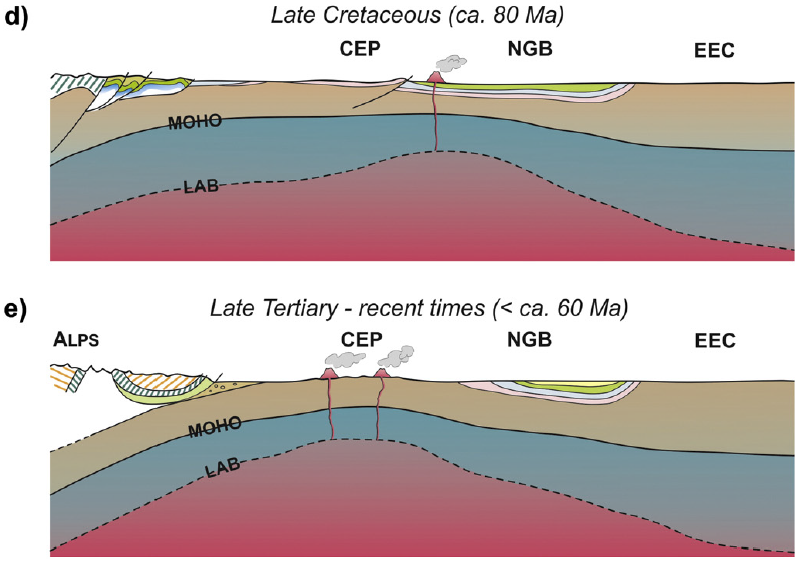
\includegraphics[width=0.5\linewidth]{../Termika/Meier2016}
	\caption{Schemat ewolucji płaszcza litosferycznego pod Europą. \textit{Na górze} późna kreda (ok. 80 mln lat temu), \textit{na dole} późny trzeciorzęd (ok. 60 mln lat temu) do dziś. \textit{CEP} platforma środkowoeuropejska, \textit{NGB} basen północnoniemiecki, \textit{EEC} kraton wschodnioeuropejski \parencite{Meier.2016}.}
	\label{meier}
\end{figure}


%McCann: https://books.google.pl/books?id=0KXptTYvKv8C&pg=PA1215&lpg=PA1215&dq=cenozoic+litosphere+heating+europe&source=bl&ots=cdGHBEBycB&sig=xHWJy_TPuji23IdjRHKsSOOAjQU&hl=pl&sa=X&ved=0ahUKEwjclJ-Xs4_bAhWI66QKHSNPDZwQ6AEIcDAM#v=onepage&q=cenozoic%20litosphere%20heating%20europe&f=false

	\section{Współczesny strumień cieplny w Europie centralnej}
	
%Dezes2004: broad thermal anomally at the base of Central European litosphere (Paleocene); prace o Islandii
%The Paleocene pre-rift injection of melilite dykes in the ECRIS area (Wilson et al., 1995) is interpreted as reflecting the activation of a mantle upwelling system beneath the Alpine foreland. (Dezes.2004)
	
	\section{Zlodowacenia plejstoceńskie}
	
Plejstocen (2,58 mln lat temu do 11,7 tys. lat temu) był czasem intensywnego rozwoju zlodowaceń na obu półkulach \parencite{Ehlers.2007}. Początek epoki lodowej, której kulminacja nastąpiła w plejstocenie \parencite{Ehlers.2007}, wyznacza pojawienie się pokrywy lodowej na wschodniej Antarktydzie ok. 35 mln lat temu (priabon --- najpó\'{z}niejszy eocen; \cite{Ehlers.2007}). Około 3 mln lat temu (pó\'{z}ny pliocen), prawdopodobnie na skutek procesów tektonicznych (m. in. zamknięcie Przesmyku Panamskiego; \cite{Driscoll.1998,Lisiecki.2007}), doszło do zmian w globalnej cyrkulacji oceaniczno-atmosferycznej \parencite{Filippelli.2009} i, w konsekwencji, ochłodzenia klimatu \ct{zrodlo}. W tych warunkach ok. 2,7 mln lat temu rozpoczęło się zlodowacenie dużych obszarów półkuli północnej, głównie w rejonach polarnych \ct{??} (ang. \textit{North Hemisphere Glaciation}; \cite{Lisiecki.2007}). Między 1,2 a 0,8 mln lat temu (blisko granicy wczesnego i środkowego plejstocenu; \cite{Head.2008}) miało miejsce stopniowe wydłużanie cyklów orbitalnych (rządzących przemiennością ciepłych i chłodnych okresów klimatycznych) z ok 41 do 100 tys. lat \parencite{Ehlers.2007,Lisiecki.2007,Head.2008}. Ekspansja ladolodu na obszary średnich szerokości geograficznych w fazach chłodnego klimatu stała sie wówczas ułatwiona \parencite{Ehlers.2007}. Region Bałtyku był pokryty lądolodem już ok. 1,1 mln lat temu, o czym świadczy m. in. charakter sedymentologiczny fluwialnej formacji Hattem (Holandia i zachodnie Niemcy), zawierającej liczne klasty pochodzenia skandynawskiego \parencite{Lee.2012}. Pierwszym zlodowaceniem, które dotarło do Niziny Środkowoeuropejskiej, było (według nomenklatury polskiej) zlodowacenie narwii \parencite{Lindner.1994} \ct{, ok. ???}, odpowiadające zlodowaceniu \ct{G\"{u}nz (Elbe???)} w nomenklaturze alpejskiej \ct{(zrodlo)}. Zlodowaceniem, które miało na ziemiach polskich największy zasięg, było zlodowacenie sanu 1 (odpowiadajace Elster II w nomenklaturze \ct{??zachodnioeuropejskiej}), które dotarło do północnego brzegu Karpat \parencite{Lindner.2001}. Maksimum ostatniego zlodowacenia (nazywanego w Polsce zlodowaceniem wisły) miało miejsce ok. 21 tys. lat temu \ct{(zrodlo)}. W tym czasie lądolód zajmował na interesującym obszarze północną część Polski, Półwysep Jutlandzki, północno-wschodnią część Niemiec i terytorium dzisiejszych państw bałtyckich \ct{(zrodlo)}. Ostatecznie z terytorium Polski lądolód ustąpił ok. 11,7 tys. lat temu \ct{(zrodlo)}.

Liczba glacjałów i interglacjałów wyznaczanych na obszarze Polski jest dyskusyjna; przyjmuje się, że w plejstocenie na terenie Polski wystąpiło 8 glacjałów i 7 interglacjałów \parencite{Lindner.1994}. Cykle klimatyczne plejstocenu Polski były korelowane z   

Zlodowacenia miały znaczny wpływ na litosferę, zwłaszcza w płytszych jej warstwach (zrodlo). Masy lodu zalegające na kontynencie europejskim powodowały znaczne obciążenie statyczne. Ciężar lądolodu, którego grubość na obszarze Polski w maksimum ostatniego zlodowacenia przekraczała 1 km \parencite{Svendsen.2004} (zrodlo), był kompensowany przez izostatyczne ugięcie skorupy na obszarze tarczy bałtyckiej (zrodlo). Śladem obciążenia litosfery przez lądolód jest [+/-] anomalia grawimetryczna, współcześnie notowana na zajmowanych przezeń w przeszłości geologicznej terenach (zrodla). Obserwuje się, zwłaszcza na Półwyspie Skandynawskim, postglacjalne wynoszenie terenu, związane z ustąpieniem lądolodu (zrodlo).

\iffalse
[...] ziemia zachowuje się jak [...] ciała plastyczne. W ciałach plastycznych deformacya nie znika razem z ciśnieniem, ale pozostaje i zanika powoli w sposób asymptotyczny. -- Rudzki, 1909 - Fizyka ziemi
\fi


Kolejnym skutkiem zlodowaceń czwartorzędowych było glacitektoniczne przeobrażenie osadów starszych oraz zdeponowanie miąższych osadów polodowcowych, tworzących charakterystyczne glacjalne formy rzeźby terenu. Grubość pokrywy osadowej ma wpływ na kształtowanie strumienia ciepła docierającego do powierzchni ziemi. Topografia terenu oraz układ warstw o różnych parametrach hydrologicznych mają zaś znaczenie dla warunków hydrologicznych – adwekcyjny i konwekcyjny transport ciepła w obrębie litosfery może zachodzić za pośrednictwem wód podziemnych.

Od samych początków współczesnych badąń geotermicznych (pierwsze dekady XX w.) zauważano (np. \cite{Stenz.1936,Rudzki.1909}) wpływ klimatu na temperaturę przypowierzchniowych warstw Ziemi. Stenz (\citeyear{Stenz.1936}) sądził, że sezonowe wahania temperatury atmosferycznej oddziałują na temperaturę gruntu do 10 m w głąb.  

Wreszcie, zlodowacenia wiązały się z przemrożeniem gruntu pod powierzchnią lodu i na obszarach tundrowych (ze względu na chłodny, surowy klimat), do głębokości kilkuset metrów pod powierzchnią gruntu, czyli z powstaniem wiecznej zmarzliny. Jako że dyfuzja termiczna w skałach odbywa się powoli, wieczna zmarzlina wciąż utrzymuje się w formie reliktowej – na kontynencie eurazjatyckim głównie na obszarze wschodniej Syberii. Reliktowy poziom wiecznej zmarzliny na obszarze Polski został udokumentowany przez badania w otworze Udryń PIG 1 w okolicy Suwałk (w roku 2010). Strop przemarzniętego poziomu znajdował się na głębokości 357 m pod poziomem gruntu. Odkrycie to jest przyczynkiem do twierdzenia, że reliktowa wieczna zmarzlina może być obecna w innych miejscach Europy środkowej i wschodniej \parencite{Szewczyk.2017}. 




 %uwzględnić, że lądolód skandynawski
 
 %kiedy był najwiekszy zasieg w europie??

%na obszar Europy lądolód wkroczył po raz pierwszy ok. 1,2 mln lat temu - sprawdzić!

%21 ka bp - last glacial maximum

\iffalse
During the Pleistocene, the Sudetes
were locally glaciated, both by mountain-type glaciers (Karkonosze
Mts., Hrubý Jeseník) as well as by a Scandinavian ice sheet advancing
from the north (Partsch, 1894; Prosová, 1973; Badura and Przybylski,
1998).

Plewa,1966: "Gdyby tak na naszych terenach zlodowacenie plejstoceńskie doszło do głębokości 300 m, to i tak w okresie kilku tysięcy lat, jakie nas dzieli od tego okresu, winna się ustalić już równowaga cieplna."

\fi
	
	
	
	\section{Orogeneza alpejska}
	
Trwająca od triasu do czwartorzędu orogeneza alpejska na obszarze Europy skutkowała powstaniem łańcuchów górskich Pirenejów, Alp, Gór Dynarskich i Karpat, oraz odmłodzeniem tektonicznym starszych jednostek. Aktywność górotwórcza następowała poprzez kolizyjną konwergencję płyt: afrykańskiej, iberyjskiej, adriatyckiej/apulijskiej \parencite{Sissingh.2006a} i subdukcję. W strefie subdukcji konsumowane były fragmenty litosfery oceanicznej, związanej z mezozoiczną ekstensją Neotetydy oraz Atlantyku (basen piemoncko-liguryski; \cite{Advokaat.2014}. Oprócz subdukcji fragmentów dna oceanicznego i konwergencji płyt: afrykańskiej i eurazjatyckiej, wydarzenia orogeniczne były w znacznej mierze kontrolowane również przez kolizje mikrokontynentów \parencite{Advokaat.2014,Dewey.1989}. W mniejszym stopniu, na kształtowanie naprężeń litosferycznych w Europie w kenozoiku wpływ miało otwieranie Atlantyku \parencite{Sissingh.2006a}. W czasie kenozoiku europejskie łańcuchy alpejskie uległy wypiętrzeniu, a przedpole orogenu alpejskiego zostało przekształcone przez wysokoamplitudowe deformacje związane z aktywnością na frontach orogenicznych.

Według Rosenbaum i in. (\citeyear{Rosenbaum.2002}), konwergencja płyt: afrykańskiej i eurazjatyckiej w kierunku północnym rozpoczęła się w pó\'{z}nej kredzie (120-67 mln lat temu; według \cite{Dewey.1989} na granicy cenomanu i turonu). Wcześniej, w pó\'{z}nej jurze i wczesnej kredzie, między Afryką a Europą funkcjonowała granica uskokowa o charakterze lewoskrętnego uskoku przesuwczego \parencite{Rosenbaum.2002,Dewey.1989}. W okresie między ok. 67-65 a 55 mln lat temu (w paleocenie) doszło do znacznego spowolnienia konwergencji \parencite{Rosenbaum.2002}. Było to prawdopodobnie spowodowane silnym spojeniem kolidujących płyt w domenie śródziemnomorskiej \parencite{Dezes.2004} oraz otwieraniem Północnego Atlantyku w procesie riftingu i powstaniem strefy uskoków transformacyjnych na granicy płyty grenlandzkiej i eurazjatyckiej \parencite{Nielsen.2007,Sissingh.2006a,Dewey.1989}. W okresie paleocenu, na ok. 10 mln lat, modus alpejskiej aktywności tektonicznej zmienił się z naprężeń powodowanych przez subdukcję tetydzkiej płyty oceanicznej na kompresję wewnątrz płyt kontynentalnych \parencite{Nielsen.2007,Sissingh.2006a}. Równocześnie (ok. 62-61 do 55 mln lat temu) z osłabieniem konwergencji, zachodnia i środkowa Europa wraz z kratonem wschodnioeuropejskim, a także Afryka północna doświadczały intensywnej kompresji wewnątrzpłytowej \parencite{Nielsen.2007,Dezes.2004}. Skutkowało to odkształcaniem litosfery oraz inwersją basenów na przestrzeni do 1700 km od głównych frontów deformacji \parencite{Dezes.2004}. Na granicy paleocenu i eocenu (ok. 55 mln lat temu) doszło do relaksacji kompresji, co nastąpiło prawdopodobnie wskutek mechanicznego odkucia alpejskiego klina orogenicznego od podłoża Po fazie kompresyjnej nastała kolejna faza nasilonej konwergencji międzypłytowej, która trwała od wczesnego eocenu, przez oligocen, po wczesny miocen (52-19 mln lat temu), z maksimum na granicy eocenu i oligocenu \parencite{Rosenbaum.2002}. W tym czasie (50-35 mln lat temu) trwała subdukcja płyty kontynentalnej \parencite{Carry.2009}. Od eocenu do pliocenu miała miejsce stopniowa dekstralna translacja na granicy kolidujących bloków litosfery (rotacja terranu Sardynii i Korsyki, a także końcowy epizod rotacji Iberii we wczesnym eocenie; \cite{Advokaat.2014,Rosenbaum.2002,Dewey.1989}). Wskutek tego, front najsilniejszych naprężeń kompresyjnych przesuwał się stopniowo ku zachodowi, z przedpola Karpat i Alp Wschodnich ku przedpolu Alp Środkowych i Zachodnich \parencite{Wilson.2006}. Przyjmuje się, że w pó\'{z}nym eocenie, kiedy nastąpiło spojenie kolidujących płyt na poziomie krustalnym, rozpoczęło się stadium pokolizyjne orogenezy alpejskiej -- przejście od subdukcji litosfery oceanicznej do kolizji płyt kontynentalnych \parencite{Sissingh.2006a}. Od pó\'{z}nego eocenu na kontynencie europejskim, w skierowanym ku północy reżimie kompresyjnym, powstawały struktury ekstensyjne związane z odmłodzeniem permo-karbońskich stref osłabień litosfery: rowy Limagne i Bresse oraz rowy reńskie \parencite{Wilson.2006}, stanowiące zaczątek rozwijającego się europejskiego systemu ryftów kenozoicznych. W pó\'{z}nym eocenie, około 35 mln lat temu, kierunek ruchu płyt dryfujących ku krawędzi platformy zachodnioeuropejskiej zmienił się z północnego na północno-zachodni \parencite{Wilson.2006,Sissingh.2006a,Dewey.1989}. Zdarzenie to łączy się \parencite{Wilson.2006,Ceriani.2001} z pó\'{z}niejszym, oligoceńskim izostatycznym dźwiganiem podłoża na przedpolu orogenu, na skutek oderwania subdukowanej płyty oceanicznej od subdukowanego fragmentu litosfery kontynentalnej w środkowych i wschodnich Alpach \parencite{Sinclair.1997,vonBlackenburg.1995}. Na oligocen przypadła główna faza rozwoju ECRIS, na skutek interferencji naprężeń kolizyjnych generowanych na frontach orogenicznych Alp i Pirenejów (np. \cite{Dezes.2004}). W miocenie współczynniki konwergencji były wciąż wysokie, ale ok. 19 mln lat temu (w burdygale) tempo konwergencji znów znacznie zmalało \parencite{Sissingh.2006a}. W warunkach wzrostu kompresji zachodziła wówczas imbrykacja zewnętrznych masywów alpejskich \parencite{Dezes.2004}. Również w burdygale rozpoczęło się wynoszenie łuku (kopuły) Wogezy-Schwarzwald, który wschodnim krańcem sięga Masywu Czeskiego \parencite{Dezes.2004}. W tortonie (ok. 10 mln lat temu, pó\'{z}ny miocen) nastąpiła wyra\'{z}na rotacja płyty afrykańskiej i Adrii/Apulii w kierunku przeciwnym do ruchu wskazówek zegara \parencite{Sissingh.2006a}. Obecnie (w pliocenie i czwartorzędzie) skracanie podłoża w zachodnich i centralnych Alpach nadal postępuje, czego dowodzi wynoszenie eksternidów alpejskich \parencite{Dezes.2004}. Obserwuje się również ciągłe d\'{z}wiganie masywów waryscyjskich (m. in. Masywu Czeskiego; \cite{Dezes.2004}) oraz neotektoniczną aktywność w obrębie ECRIS (zrodlo). Na kontynencie europejskim (w jego zachodniej i centralnej części) panuje skierowany ku N-NW reżim kompresyjny, co Dezes i in. (\citeyear{Dezes.2004}) przypisują: 1) obrotowi Afryki i Arabii względem Eurazji przeciwnie do ruchu wskazówek zegara; 2) interakcji kolizyjnej Europy z klinem alpejskim; 3) rozrostowi dna oceanicznego Północnego Atlantyku.

%czy mozna powiedzieć "konwergencja w kierunku północnym"?
%Adria=+/-N część Apulii
%koniecznie dopisać o Adrii + ccw rotacji Adrii/Apulii!! i może o Dynarydach (spr ich zasięg)

	\subsection{Wypiętrzenie Karpat}
	
%Golonka
%odw. do cyklu Wilsona
	
	\subsection{Powstanie systemu ryftów na kontynencie europejskim}
	
%Sissingh.2006a
	
Wykształcenie się w kenozoiku systemu ryftów i uskoków przecinających wszystkie waryscyjskie masywy na przedpolu Alp (ang. ECRIS -- \textit{European Cenozoic Rift System}, Fig. \ref{dezes}) było prawdopodobnie spowodowane reakcją hercyńskiego podłoża na akrecję bloków kontynetalnych podczas orogenezy alpejskiej \parencite{Ulrych.2002}. U początków eocenu naprężenia kompresyjne na przedgórzu Alp (konwergencja Europy i Adrii-Apulii; np. \cite{Sissingh.2006a}) zmniejszały się względem naprężeń powodujacych fałdowanie Pirenejów (konwergencja na granicy Europa-Iberia; \cite{Rosenbaum.2002}) wskutek czego (kiedy? we wczesnym/poznym eocenie?) doszło do otwarcia systemu ryftów w międzypłytowym reżimie kompresyjnym (\cite{Ziegler.2007}; \cite{Dezes.2004}). Lokalizacja kenozoicznych ryftów była powiązana z wcześniejszym, permo-karbońskim systemem spękań na kontynencie europejskim \parencite{Wilson.2006,Sissingh.2006a}. Zwłaszcza od przełomu eocenu i oligocenu rozwój ryftów kontrolowany był przez ponadregionalny E-W reżim ekstensyjny, który miał wpływ na reżim naprężeń w domenie alpejsko-śródziemnomorskiej \parencite{Sissingh.2006a}. Główna faza riftingu przypadła na oligocen, kiedy to proces ten był kontrolowany przez działające w kierunku północnym naprężenia powstające w strefach kolizyjnych Alp i Pirenejów (zrodlo?). Od wczesnego miocenu, po ustaniu subdukcji w Pirenejach i otwarciu basenu algiersko-prowansalskiego w zachodniej części Morza Śródziemnego, rozwój ECRIS był podtrzymywany przez naprężenia oddziaływujące w kierunku północnym i północno-zachodnim związane z powstawaniem eksternidów alpejskich \parencite{Dezes.2004}. Uniesienie astenosfery (w rodzaju pióropusza płaszcza) pod ścienioną litosferą alpejskiego przedpola umożliwiło rozpoczęcie wytapiania zmetasomatyzowanego płaszcza \parencite{Ulrych.2002} oraz spowodowało jej mechaniczne osłabienie, powodując podatność na deformację \parencite{Dezes.2004}. Aktywność tektoniczna związana z ryftowaniem oraz wulkanizm w rowach należących do ECRIS wygasały w różnym czasie. Rowy Masywu Centralnego i Rodanu stały się nieaktywne z początkiem miocenu, podczas gdy system rowów reńskich wykazuje aktywność do dzisiaj \parencite{Dezes.2004}. Najbardziej wysuniętym na wschód i jednocześnie najbliższym terytorium Polski jest ryft Egeru.

%Advokaat -- sprawdzić!
%roll-back a ekstensja

\begin{figure}[h]
	\centering
	\includegraphics[width=0.7\linewidth]{../Termika/dezes2004}
	\caption{Rozmieszczenie rowów tektonicznych (\textit{jasnoszary}) powstałych w kenozoiku na przedpolu Alp i Pirenejów oraz związanych z nimi pól wulkanicznych (\textit{czarny}), linia przerywana -- front deformacji alpejskich; \textit{BF} Schwarzwald, \textit{BG} rów Bresse, \textit{EG} rów Eger, \textit{FP} Wyżyna Frankońska, \textit{HG} rowy heskie, \textit{LG} rów Limagne, \textit{LRG} rów Dolnego Renu, \textit{URG} rów Górnego Renu, \textit{OW} Odenwald, \textit{VG} Wogezy \parencite{Dezes.2004}.}
\label{dezes}
\end{figure}

Według D\`{e}zes i in. (\citeyear{Dezes.2004}), ryftowanie w obrębie ECRIS przebiegało w następujących fazach: 
\begin{enumerate}[nolistsep]
	\item faza przedryftowa (paleocen -- środkowy eocen);
	\item wczesna faza riftingu (pó\'{z}ny eocen);
	\item główna faza riftingu (oligocen -- najstarszy miocen);
	\item pó\'{z}na faza riftingu (pó\'{z}ny akwitan -- pliocen).
\end{enumerate}

%syn- i post-rift -- jakie byly te fazy w przypadku ECRIS

\subsubsection{Ryft Egeru}

Ryft Egeru (Oh\v{r}y) powstał w fazie ekstensji, która dotknęła Masyw Czeski na przestrzeni od eocenu do miocenu (zrodlo). Trzeciorzędowy ryft powstał w miejscu waryscyjskiego szwu między jednostką saksoturyngijską a Tepl\`{a}-Barrandien \parencite{Mlcoch.2012}, będącego wschodnim przedłużeniem kontaktu między tą drugą jednostką a jednostką mol-danubską \parencite{Plomerova.2007}. Powstanie ryftu Egeru było wynikiem dwóch faz ekstensyjnych \parencite{Haloda.2012}: 1) pó\'{z}ny eocen -- wczesny miocen: ekstensja w kierunkach NNE-SSW do N-S, skośnie do osi ryftu, prawdopodobnie w związku z termicznym wynoszeniem (\textit{thermal doming}) Masywu Czeskiego. Efektem tej fazy był silny magmatyzm typu OIB w granicach ryftu; 2) ortogonalna ekstensja związana z rozciąganiem wzdłuż osi regionalnego antyklinorium, powstałego prawdopodobnie jako przejaw fałdowania na przedpolu alpejsko-karpackim. Kierunki ekstensji w tym modelu przypominają orientacje ortogonalnych systemów nieciągłości tektonicznych obserwowanych w strefie Żytawa-Siekierczyn \parencite{Piatkowska.2000}. Roz-mieszczenie intruzji magmowych w rowie Egeru świadczy o postępującym ku wschodowi rozwoju ryftu. Ostatni etap rozwoju ryftu przypadł na 24-16(?) mln lat temu (pó\'{z}ny oligocen -- miocen) i był to czas kształtowania się współcześnie obserwowanej struktury rowu ograniczonego przez uskoki \parencite{Adamovic.1999} --- od południa przez strefę uskokową Czeskiego Średniogórza, a od północy przez strefę uskokową Rudaw \parencite{Cajz.2012}. Subsydencja rowu Egeru, która rozpoczęła się pod koniec pó\'{z}nooligoceńskiego pulsu magmatycznego, odbywała się prawdopodobnie w dużej mierze pod wpływem lokalnego pola naprężeń, związanego z kolapsem kopuły termicznej \parencite{Dezes.2004}.

 Wulkanizm rozwijał się współcześnie z intensywną subsydencją i sedymentacją w ryfcie, w wyniku której doszło do nagromadzenia miąższych osadów miocenu morskiego \parencite{Grygar.2016}.

Z powstaniem ryftu Egeru wiązała się intensywna działalność wulkaniczna w kenozoiku. W wyniku tej aktywności, w granicach ryftu powstało wiele pól wulkanicznych, z których największe to Doupovsk\'{e} hory (\cite{Haloda.2012}; \cite{Skacelova.2009}) i Czeskie Średniogórze (\cite{Cajz.2009}; Fig. \ref{cajz}). Wulkanizm rozwijał się wzdłuż uskoków, zwłaszcza tych ograniczjących ryft od południowego wschodu \parencite{Grygar.2016}. Ponadto, produkty działalności wulkanicznej w ryfcie Egeru na jego północno-wschodnim krańcu (sięgającym terytorium Polski) znajdowane są na obszarze masywu łużyckiego i zaliczanych do strefy obniżeń Żytawa-Siekierczyn depresji: niecki żytawskiej, niecki berzdorfsko-radomierzyckiej, basenu Siekierczyna, basenu Fr\'{y}dlant-Vianov\'{a} (\cite{Woloszyn.2017}; \cite{Cajz.2009}; \cite{Piatkowska.2000}). 

%wiek tych pol wulk?

\begin{figure}[h]
	\centering
	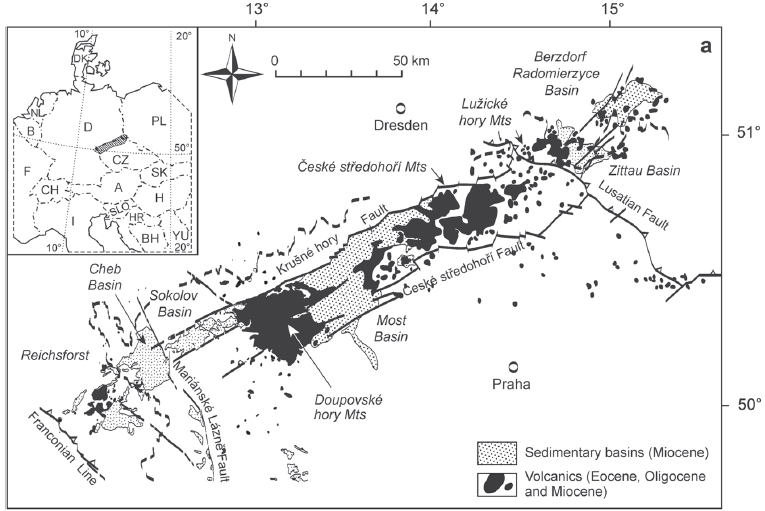
\includegraphics[width=0.7\linewidth]{C:/Users/Agata_P/Documents/Termika/Termika/ryft_egeru.png}
	\caption{Szkic tektoniczny ryftu Egeru z zaznaczonymi miejscami występowania wulkanitów kenozoicznych \parencite{Cajz.2009}.}
	\label{cajz}
\end{figure}

%sprawdzić te nazwy stref uskokowych po polsku

	\subsection{Wynoszenie masywów waryscyjskich}
	
W kenozoiku, oprócz ryftowania, dochodziło na kontynencie europejskim do wynoszenia waryscyjskiego podłoża na przedpolu Alp. Za proces ten odpowiedzialne były w dużej mierze te same czynniki, które doprowadziły do powstania ECRIS. Miejscami wynoszenie podłoża zaczęło się już pod koniec kredy, wyra\'{z}nie przyśpieszyło w miocenie i trwa do dziś. Czynnikami powodującymi d\'{z}wiganie waryscyjskiego podłoża był stres kompresyjny związany z kolizją alpejską oraz aktywność pióropuszów płaszcza (\cite{Ziegler.2007}; \cite{Wilson.2006}; \cite{Wilson.2001}). W tych warunkach dochodziło do powstawania kopułowatych wyniesień w miejscach przegrzania osłabionej litosfery (ang. \textit{thermal doming}). Na obszarze Europy centralnej najbliższą jednostką tego typu jest Masyw Czeski, na którego północno-wchodnim krańcu, na terenie Polski znajdują się kopuły: orlicko-śnieżnicka, Desny, wschodniosudecka, Kerpnika i karkonosko-izerska (\cite{Cymerman.2016}; \cite{Mazur.2001}; \cite{Maluski.1995}). 

Wynoszone w kenozoiku fragmenty starszego podłoża były poddane przeobrażeniom tektonicznym i termicznym podczas orogenezy waryscyjskiej, z tego względu są to fragmenty skorupy o cieńszej litosferze i wyższym strumieniu cieplnym niż otaczające kratony. Czynniki te prawdopodobnie umożliwiły rozwój pól wulkanicznych na tych obszarach w kenozoiku \parencite{Wilson.2006}.

%Sobczyk et al., 2015 (czy tutaj?)

%Vosges-Black Forest arch(dome)

		\subsubsection{Masyw Czeski}

Masyw Czeski, zajmujący obszar zachodnich i środkowych Czech, zaczął się kształtować w paleoproterozoiku (ok. 2 mld lat temu). Strukura ta powstała w wyniku scalenia czterech mniejszych bloków litosfery --- jednostek: moldanubskiej, Tepl\'{a}-Barrandien, saksoturyńskiej i morawsko-śląskiej. Jednostka sakso-turyngijska podzielona jest młodszą strefą uskokową Łaby na strefe Rudaw i strefę zachodniosudecką lub Lugicum \parencite{Grygar.2016}. Pod względem litologii i geofizycznych właściwości skorupy i płaszcza oraz historii metamorficznej wyróżnia się jednostka moldanubska \parencite{Grygar.2016}. Litosfera Moldanubicum osiąga miąższości 120-140 km i jest grubsza od litosfery jednostki saksoturyngijskiej (90-120 km; \cite{Babuska.2001}). Jako homogeniczna jednostka masyw ten zaczął funkcjonować w wyniku aktywności tekonicznej we względnie wczesnych fazach orogenezy waryscyjskiej (wczesny westfal; \cite{Grygar.2016}). Masyw Czeski został włączony w obręb orogenu waryscyjskiego (internidy waryscyjskie); jego tektoniczne odmłodzenie i wyniesienie nastąpiło wraz z orogenezą alpejską. Wynoszenie północnej części masywu rozpoczęło się w miocenie (burdygał) i trwała przez pliocen oraz czwartorzęd \parencite{Dezes.2004}. Subdukcyjne zamknięcie basenu piemoncko-liguryjskiego w domenie wschodnioalpejskiej i w północnych Karpatach skutkowało kolizją austroalpejskiego klinu orogenicznego z kontynentem europejskim, czego konsekwencją było wyniesienie Masywu Czeskiego oraz inwersja bruzdy śródpolskiej \parencite{Dezes.2004}.

Na podstawie badań traków w apatytach i datowania na cyrkonach z próbek z Rudaw Janowickich ustalono \parencite{Sobczyk.2015}, że w środkowej kredzie rejon ten znajdował się w warunkach pogrzebania i temperatur ok. 190 \textcelsius. W kenozoiku (od cenomanu) północna część Masywu Czeskiego uległa ekshumacji (3,3-3,5 km wyniesienia; \cite{Sobczyk.2015}). 

W kenozoiku Masyw Czeski doświadczył kilku faz wulkanizmu. W paleocenie doszło do iniekcji stopów melilitytowych, które genetycznie powiązane były z aktywacją upwellingu płaszczowego na przedpolu Alp \parencite{Dezes.2004}. Obszar Masywu doświadczał następnie aktywności wulkanicznej w czasie eocenu (zwłaszcza pod koniec tego okresu),  we wczesnym i środkowym oligocenie, w miocenie (ze stopniowym wygaszaniem ku końcowi miocenu) oraz w pliocenie i czwartorzędzie \parencite{Dezes.2004}. 


	
	
	\subsection{Powstanie zapadlisk przed- i śródgórskich}
	
Wypiętrzeniu Karpat towarzyszyło powstanie rejonów zapadliskowych, do których zalicza się zapadlisko przedkarpackie i basen panoński. Ograniczony łańcuchami Alp, Karpat i Gór Dynarskich basen panoński (Fig. \ref{kovac}) dzieli się na wiele podjednostek, z których największą i centralną jest obniżenie Wielkiej Niziny Węgierskiej. Oprócz Wielkiej Niziny Węgierskiej, do panońskiego systemu basenów należą również mniejsze baseny, m. in. basen dunajski (Mała Nizina Węgierska), basen Grazu (styryjski), których granice wyznaczają masywy gór wyspowych. Baseny znajdujące się na obrzeżach domeny panońskiej (basen wiedeński, transylwański, transkarpacki) położone są w bezpośrednim sąsiedztwie granicy płaszczowin eoalpejskich (występujących w podłożu basenu panońskiego) oraz nasunięć fliszu karpackiego (\cite{Kovac.2007}; \cite{Fodor.1999}).

\begin{figure}[h]
	\centering
	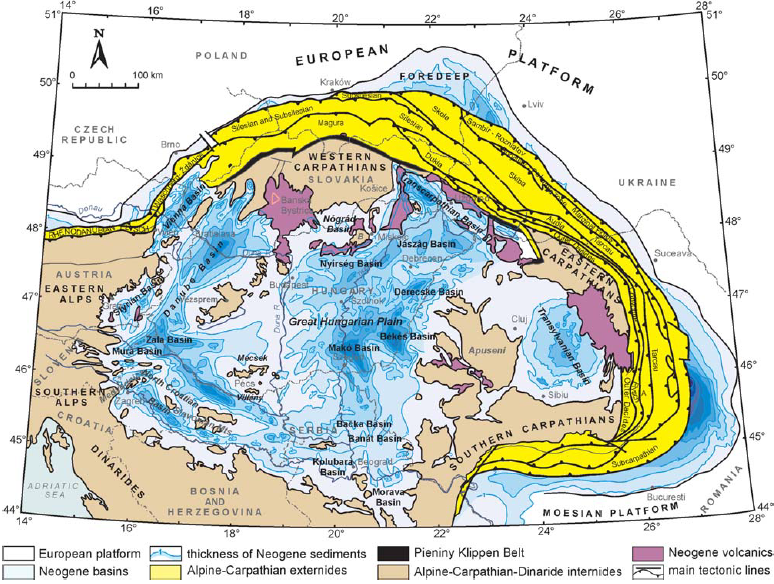
\includegraphics[scale=0.7]{C:/Users/Agata_P/Documents/Termika/Termika/kovac.png}
	\caption{Jednostki georegionalne w otoczeniu basenu panońskiego \parencite{Kovac.2007}.}
	\label{kovac}
\end{figure}



		\subsubsection{Basen panoński}

Panoński system basenowy powstał w wyniku serii zdarzeń tektonicznych, mających miejsce od środkowego triasu do dziś. W mezozoiku obszar współczesnego basenu panońskiego wypełniał ocean Neotetydy, w którego podłożu rozwijały się strefy ryftowe. Pod koniec jury doszło do zderzenia terranów Alcapa i Tisza-Dacja, których kontakt współcześnie wyznacza śródwowęgierska strefa uskokowa. Utworzone wówczas płaszczowiny stanowią podłoże współczesnego basenu panońskiego \parencite{Csontos.2004}. Od eocenu (kolizja kontynent-kontynent w regionie alpejskim) rozwijała się ku wschodowi karpacka strefa subdukcji. W miocenie rozpoczęła się faza ekstensji basenu w jego wewnętrznych partiach, jednocześnie z aktywnością subdukcyjną w strefach brzeżnych \parencite{Csontos.2004}. Około 20 mln lat temu (w burdygale) rozpoczęła się rotacja (w kierunku przeciwnym do ruchu wskazówek zegara) i subdukcja Adrii pod alpejski klin orogeniczny. W tej sytuacji tektonicznej, wertykalne rozrywanie Adrii doprowadziło do uniesienia astenosfery i termicznej erozji litosfery północnych Dynarydów. Odkucie litosfery od płaszcza ułatwiło subdukcję (typu \textit{rollback}) w domenie karpackiej, i, w konsekwencji, ekstensję basenu panońskiego \parencite{Handy.2012}. Po etapie intensywnej ekstensji dalszy rozwój basenu następował na drodze subsydencji termicznej, będącej efektem kontrakcji termicznej litosfery podczas jej stygnięcia. Taki dwuetapowy model rozwoju basenu ekstensyjnego (faza intensywnej ekstensji, a po niej bardziej pasywna faza subsydencji) potwierdzają badania sejsmiki refleksyjnej i luster tektonicznych w uskokach na obszarze basenu panońskiego. Obecnie (od pó\'{z}nego pliocenu) teren basenu panońskiego znajduje się w reżimie kompresyjnym, w którym jego brzeżne partie na wschodzie i zachodzie ulegają wynoszeniu \parencite{Horvath.1996}. 

%napisać o rotacji w eocenie - zrodla w harangi i lenkey 2007

Basen panoński charakteryzuje się cienką litosferą (50-80 km) i skorupą (22-30 km; \cite{Harangi.2007}; Fig. {horvath}). Litosferę basenu panońskiego cechują wyjątkowo wysokie wartości strumienia cieplnego, przekraczające 80 \si{\milli\watt\per\meter\squared} \parencite{Boldizsar.1964}. Mierzone wartości strumienia cieplnego mieszczą się w przedziale 50-130 \si{\milli\watt\per\meter\squared}, a średnia wynosi okolo 100 \si{\milli\watt\per\meter\squared} \parencite{Horvath.2015}. Takie warunki termiczne są pozostałością po mioceńskim etapie ekstensji, w trakcie którego doszło do silnego wygrzania litosfery \parencite{Lenkey.2017}. Ze zjawiskami termicznymi związany był neogeńsko-czwartorzędowy (21-0,1 mln lat temu) wulkanizm o charakterze kwaśnym i kalcialkalicznym. W czasie geologicznym wulkanizm ten migrował z zachodu na wschód \parencite{Lexa.2010}. 

Największe wartości strumienia cieplnego rejestrowane są w miejscach wyniesień podłoża między głębszymi basenami Wielkiej Niziny Węgierskiej \parencite{Bekesi.2017}. 

\begin{figure}[h]
	\centering
	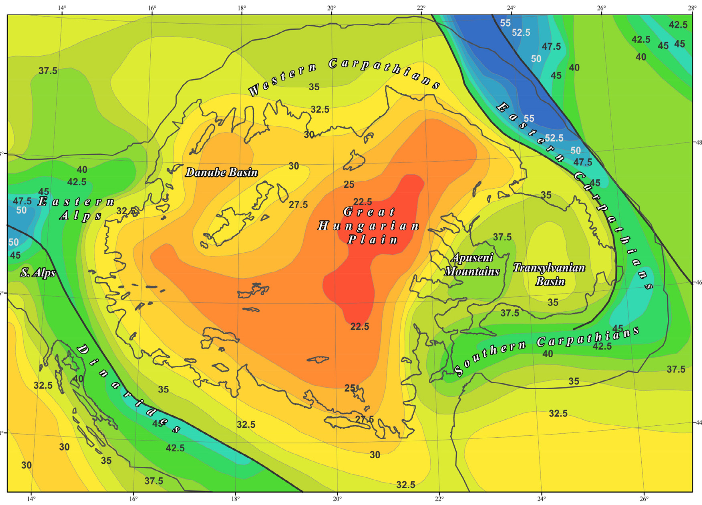
\includegraphics[width=0.7\linewidth]{C:/Users/Agata_P/Documents/Termika/Termika/grubosc_skorupy.png}
	\caption{Rozkład grubości skorupy w regionie panońskim \parencite{Horvath.2015}.}
	\label{horvath}
\end{figure}

 W związku ze znaczną subsydencją, basen panoński był miejscem intensywnej sedymentacji, w wyniku której doszło do nagromadzenia miąższych (0,1-7 km) osadów neogeńskich, o~charakterze morskim, deltowym, jeziornym i rzecznym \parencite{Toth.2001}. Intensywna sedymentacja jako proces oraz sposób występowania warstwy osadowej w profilu geologicznym mają istotny wpływ na kształtowanie strumienia cieplnego docierającego do powierzchni ziemi. Wysokie tempo sedymentacji zmniejsza wartości strumienia cieplnego rejestrowane przy powierzchni ziemi (\cite{Lenkey.2017}; \cite{Horvath.2015}). Wartości strumienia cieplnego z poprawką na sedymentację są o 10-30 \% wyższe od bezpośrednio obserwowanych \parencite{Lenkey.2002}. Ponadto, skały osadowe są środowiskiem występowania zjawisk hydrogeologicznych, które mają pewien wpływ na strumień cieplny. Infiltracja wód meteorycznych (szczególnie w miejscach wychodni powierzchniowych wysoko porowatych wapieni) przyczynia się do znacznego spadku rejestrowanych wartości strumienia cieplnego, np. w Dynarydach zewnętrznych do 30 \si{\milli\watt\per\meter\squared} \parencite{Horvath.2015}. Ogrzane wody meteoryczne docierając z powrotem ku powierzchni ziemi odpowiadają za powstawanie gorących \'{z}ródeł, licznie występujących na obszarze panońskim. Pomiar energii termicznej niesionej przez gorące wody może posłużyć do oszacowania konwekcyjnego transportu ciepłą, a dodanie tej wartości do obserwowanego strumienia cieplnego daje w wyniku wartość strumienia cieplnego w warunkach niezaburzonych przez cyrkulację wód \parencite{Lenkey.2017}. Cyrkulacja wód podziemnych jest również przyczyną zaburzeń kondukcyjnego przepływu ciepła płaszczowego ku powierzchni ziemi. Grawitacyjny przepływ wód podziemnych oraz rozwijanie się komórek konwekcyjnych w obrębie tych wód mogą zmienić wartości powierzchniowego strumienia cieplnego \parencite{Horvath.2015}. 
 
 W obrębie wypełnienia osadowego basenu panońskiego (neogeńskiego i mezozoicznego) wykształciły się dwa systemy wodonośne, przedzielone warstwą oligoceńskich osadów marglistych o niskiej przepuszczalności. W wyższym systemie dominujący czynnik powodujący przepływ jest natury grawitacyjnej, związany z topografią. Niższy system (cyrkulacja w skałach położonych głębiej) poddany jest oddziaływaniom tektonicznym o charakterze kompresyjnym, które są przyczyną wytworzenia nadciśnienia w wodach porowych \parencite{Toth.2001}. Innym wytłumaczeniem takiego stanu rzeczy jest duże tempo sedymentacji, niezrównoważone z tempem kompakcji i odprowadzania wód porowych, przez co ciśnienie w wodach porowych danego ośrodka narasta \parencite{Horvath.2015}. Oba systemy nie są w pełni izolowane, jako że uskoki stanowią miejsca ułatwionego przepływu solanek z niższego systemu ku powierzchni \parencite{Toth.2001}. Mezozoiczne formacje węglanowe z wychodniami na powierzchni ziemi stanowią odrębny system hydrogeologiczny z przzepływem kontrolowanym grawitacyjnie \parencite{Horvath.2015}. 
 
 Wysokie ciśnienia i temperatury panujące w obrębie skał niższego systemu wodonośnego, w połączeniu z dużą porowatością tych utworów, umożliwiają rozwój konwekcyjnego przepływu wód \parencite{Horvath.2015}.
 
 %Handy et al., 2012
 
	\paragraph{Basen wiedeński}

Basen wiedeński jest jednostką stosunkowo chłodną (izoterma 100 \textcelsius znajduje się na głębokości poniżej 2500 m), ale jako basen sedymentacyjny może w przyszłości stanowić dogodne \'{z}rodło energii geotermalnej \parencite{Hoyer.2012}.

%Holzel et al., 2008
 
 \subsubsection{Zapadlisko przedkarpackie}
 
 \subsubsection{Alpejski basen molasowy}
 
 Alpejski basen przedpola, rozciągający się na północ i zachód od łuku Alp, powstał w pó\'{z}nym paleocenie w wyniku fleksuralnego ugięcia litosfery w strefie konwergencji wzdług pasywnego brzegu platformy zachodnioeuropejskiej, pod ciężarem rozwijającego się klinu orogenicznego Alp \parencite{Sissingh.2006a}. W pó\'{z}nym eocenie, wraz z rozbudową alpejskiego klina orogenicznego, nastąpiło szybkie poszerzenie basenu \parencite{Dezes.2004}.
 
 
 
 \iffalse
 Sissingh.2006a: Earlier, structurally important phases of foreland compression
 occurred in the Paleocene. Through Late Paleocene intra-plate
 compression, Laramide and older features of the continental
 Alpine foreland were uplifted and degraded by erosion, whereas
 farther to the south, the development of the Alpine Foreland
 Basin was initiated by load-induced downflexing of the prowedge
 foreland crust by the nascent Alpine orogenic wedge
 (Allen et al., 1991).
 \fi
 
 \iffalse
  W pó\'{z}nym eocenie, około 35 mln lat temu, kierunek ruchu płyt dryfujących ku krawędzi platformy zachodnioeuropejskiej zmienił się z północnego na północno-zachodni \parencite{Wilson.2006,Sissingh.2006a,Dewey.1989}. Jak zaznaczają \cite{Wilson.2006} i \cite{Ceriani.2001}, zdarzenie to nastąpiło w interesującej koincydencji ze zmianą charakteru sedymentacji w alpejskim basenie molasowym (alpejskim basenie przedpola) w czasie oligocenu. Przejście z głębokowodnego do płytkowodnego typu sedymentacji mogło być związane z izostatycznym dźwiganiem podłoża basenu na skutek oderwania subdukowanej płyty oceanicznej od subdukowanego fragmentu litosfery kontynentalnej \parencite{Sinclair.1997,vonBlackenburg.1995}.
  \fi
 
 %Krzywiec, 2006
 %alpejski basen molasowy
 %Gusterhuber et al., 2012
 %Andeweg i Cloetingh, 1998
 %the Molasse Basin
 %Anczkiewicz et al., 2013
 %Kuhlemann i Kempf, 2002
 %Sinclair, 1997
 
 \section{Wulkanizm}
 
 Zjawiska wulkaniczne są zarówno bezpośrednią przyczyną podwyższenia lokalnej charakterystyki termicznej, jak i przejawem regionalnych fenomenów natury litosferycznej czy płaszczowej (odpowiedzialnych za wulkanizm), wpływających na wartości parametrów termicznych na danym obszarze. Bepośredni wpływ wulkanizmu na temperaturę litosfery wyraża się w powstawaniu aureoli termicznych wokół ciał magmowych intrudujących w skały górotworu. Dokładna ilościowa ocena wpływu termicznego intruzji na otaczający górotwór musi uwzględniać wiele czynników, m. in. geometrię ciała magmowego, różnice w przewodności cieplnej ośrodków, konwekcję w magmie, możliwość zainstnienia konwekcji wód porowych w skałach otoczenia; w mniejszym stopniu reakcje metamorficzne (dehydratacja, rozkład węglanów i inne) czy wolatylizację wód porowych \parencite{Annen.2017}. Wpływ termiczny intruzji na skały otoczenia zanika w następujący sposób \parencite{Majorowicz.1975}:
 
 \begin{itemize}
 	\item dla intruzji o geometrii warstwy grubości \(2d\): \\
 	\[\Delta T_{p} = d \Delta T_{0}{(\Pi\kappa{t})}^{-\frac{1}{2}}\] \\
 	
 	\item dla intruzji o geometrii kulistej i promieniu \(d\):
 	\[\Delta T_{p} = \frac{1}{6}\Pi{d^{3}}{\Delta T_{0}}{(\Pi \kappa{t})}^{-\frac{3}{2}}\]\\
 	\\
 	gdzie: \\
 	\(\Delta T_{0}\) --- początkowa różnica temperatur między skałami otoczenia a intruzją, \\
 	\(\Delta T_{p}\) --- różnica temperatur między skałami otoczenia a intruzją po czasie t, \\
 	\(\kappa = K/\rho{c}\), gdzie: \(K\) --- przewodność cieplna, \(c\) --- pojemność cieplna.
\end{itemize}
 
\noindent Według powyższych wzorów, intruzja o geometrii płyty wychładza się dziesięciokrotnie w czasie 0,5--0,25 mln lat, a intruzja o geometrii kulistej --- w czasie 0,31 mln lat \parencite{Majorowicz.1975}.	
 
 Grubość aureoli wokół intruzji odzwierciedla dynamikę tworzenia intruzji --- w wyniku pojedynczego zdarzenia bąd\'{z} na drodze wieloetapowego procesu \parencite{Galushkin.1997}. Wpływ termiczny intruzji na skały otoczenia może być ewaluowany w badaniach refleksyjności witrynitu (jako miernika przetworzenia termicznego materii organicznej; np. \cite{Annen.2017}; \cite{Fjeldskaar.2008}). Warunki termiczne panujące w \'{z}ródle, gdzie generowana jest magma (płaszczowe bąd\'{z} skorupowe) oraz tempo migracji magmy mogą być oceniane na podstawie badań inkuzji (np. gęstość CO$_{2}$, \cite{Ladenberger.2009}) lub składu chemicznego minerałów w ksenolitach (zrodlo). Stosunki zawartości pierwiastków w różnych minerałach, np. w dwóch piroksenach (termometr piroksen-piroksen??), mogą posłużyć do obliczenia temperatur zamknięcia systemu (zrodlo). \ct{wszędzie powt. "mogą"}
 
 Wulkanizm kenzoiczny w Europie występuje w dwóch głównych środowiskach geotektonicznych, w odniesieniu do orogenezy alpejskiej: anorogenicznym i orogenicznym \parencite{Wilson.2006}. W Europie środkowej wulkanizm anorogeniczny w kenozoiku przejawia się w miejscach związanych z ECRIS i synchronicznie wyniesionymi masywami waryscyjskimi (Sudety, ryft Egeru, a dalej na zachód, na obszarze Niemiec - m. in. Vogelsberg, depresja północnoheska, Eifel). Wulkanizm typu orogenicznego, współczesny z subdukcją, był w rejonie Europy centralnej obecny na obszarze Karpat (w Polsce: Pieniny; \cite{Badura.2004}) i basenu panońskiego. 
 
 \subsubsection{Wulkanizm karpacki i panoński}
 
 Na obszarze poddanym przekształceniom podczas orogenzey alpejskiej pojawiły się w kenozoiku związane genetycznie z procesami górotwórczymi zjawiska wulkaniczne. Alpejskie wydarzenia orogeniczne kredy i paleogenu, kiedy miało miejsce skracanie litosfery oceanicznej Oceanu Tetydy na drodze subdukcji, nie skutkowały w tym czasie zjawiskami wulkanicznymi w domenie karpacko-panońskiej. Przyczyną tego był panujący wówczas na tym obszarze reżim kompresyjny oraz znaczna grubość litosfery, niepoddanej jeszcze wówczas ekstensji. Jednakże, zaistniała wówczas metasomatyzacja płaszcza, możliwa dzięki dehydratacji subdukowanych fragmentów litosfery. Uwodnienie płaszcza pozwoliło na zmniejszenie temperatury generacji stopu, który zaczął migrować ku powierzchni wraz z rozpoczęciem etapu ekstensji we wczesnym miocenie, około 20 mln lat temu. Stopy płaszczowe, docierając do skorupy, powodowały jej topnienie i tworzenie magm krustalnych. W etapie ekstensji generacja magm płaszczowych podtrzymywana była przez mechanizm wytapiania dekompresyjnego, a dalsza subdukcja wpływała na skład magm i umożliwiała obniżenie temperatury likwidusu \parencite{Harangi.2007}. Oprócz wulkanizmu związanego z subdukcją (orogenicznego), w domenie karpacko-panońskiej występowały lokalnie pó\'{z}niejsze zjawiska wulkaniczne natury anorogenicznej \parencite{Wilson.2006}.
 
 %zob. Konecny et al., 2002   
 
 Wulkanizm kenozoiczny (neogeński) domeny karpacko-panońskiej był fenomenem wieloetapowym. Kolejne jego fazy cechowały się różnym chemizmem oraz miejscem występowania. Ogółem, zjawiska te datowane są na okres 21-0,1 mln lat temu, przy czym centrum aktywności wulkanicznej przesuwało się w czasie z zachodu na wschód (\cite{Lexa.2010}; \cite{Pecskay.1995}). Zmienny charakter chemiczny zjawisk wulkanicznych odzwierciedlał różne epizody tektoniczne w rejonie. Wyróżnia się trzy główne etapy wulkanizmu karpacko-panońskiego w neogenie: 1) miocen (około 20-11 mln lat temu): kwaśny wulkanizm kalcialkaliczny --- ignimbryty i tufy basenu panońskiego i transylwańskiego; 2) środkowy miocen - czwartorzęd (17-0,2 mln lat temu): pośredni (między felsytowym a maficznym) wulkanizm kalcialkaliczny (niezwiązany genetycznie z wulkanizmem felsytowym miocenu), z końcową fazą bazaltową --- andezyty (w tym andezyty pienińskie) występujące w łuku wulkanicznym po wewnętrznej stronie Karpat fliszowych, rozciągającym się od basenu dunajskiego po rumuński kompleks Călimani-Gurghiu-Harghita; 3) wulkanizm alkaliczny (dwie fazy: 17-7 i 6-0,5 mln lat temu) --- sporadyczne wystąpienia na całym obszarze karpacko-panońskim --- od szoszonitów kapratu (17-16 mln lat temu) do bazaltów alkalicznych i szoszonitów czwartorzędowych \parencite{Pecskay.1995}.
 
 Geneza zjawisk wulkanicznych w regionie Karpat i basenu panońskiego w oczywisty sposób wydaje się być powiązana z historią tektoniczną tego obszaru. Kwestią dyskusji jest, czy współcześnie obserwowane wysokie wartości parametrów termicznych związane są z postulowanym przez niektórych badaczy (np. \cite{Wilson.2001}) pióropuszem płaszcza w podłożu panońskim. Sygnatury izotopowe HIMU i FOZO, którymi charakteryzują się alkaliczne skały magmowe basenu panońskiego i Karpat oraz charakterystyka termiczna regionu przemawiają za hipotezą istnienia pióropusza. Jednakże, taki skład izotopowy może być efektem metasomatozy (niekoniecznie zaś pióropusza płaszcza), a wysokie wartości strumienia cieplnego wyjaśnia również ścienienie skorupy podczas ekstensji i płytkie usytuowanie LAB (ang. \textit{litosphere-astenophere boundary}). Wpływ epizodu ekstensyjnego na wartości strumienia cieplnego wygasa po ok. 100 milionach lat (McKenzie, 1978 --> znalezc), więc w płaszczu pod basenem panońskim wciąż mogą istnieć warunki do generacji stopu (prawdopodobnie w wyniku podwyższenia temperatury przez inną niż piórpusz płaszcza nieokreśloną perturbację natury płaszczowej). Przeciwko hipotezie pióropusza płaszcza pod basenem panońskim przemawia także brak kopułowatego wyniesienia regionu w topografii, sporadyczny charakter i rozproszenie przestrzenne przejawów wulkanizmu panońskiego oraz niskie tempo produkcji magmy \parencite{Harangi.2007}.    
 
 Wpływ intruzji na zwiększenie temperatur i strumienia cieplnego w ich pobliżu wygasa w ciągu kilku do kilkudziesięciu milionów lat (\cite{Lenkey.2002,Majorowicz.1975}). Anomalnie wysokie wartości strumienia cieplnego na obszarze Karpat Wschodnich mogą być wiązane z zakończoną około 0,1 miliona lat temu aktywnością wulkaniczną na tym obszarze. Śródkowomioceński wulkanizm kalcialkaliczny i zjawiska wulkaniczne występujące w przeszłości wzdłuż łuku Karpat po jego wewnętrznej stronie nie powinny mieć więc współcześnie wpływu na podwyższenie parametrów termicznych. Emisja ciepła radiogenicznego z powstałych wówczas utworów wulkanicznych, z uwagi na względnie małą zawartość pierwiastków promieniotówrczych, nie ma istotnego wpływu ilościowego na strumień cieplny. Obserwowane wysokie wartości temperatur i strumienia cieplnego mają więc zapewne \'{z}ródło w dolnej skorupie bąd\'{z} płaszczu; domniemywać można, że to samo \'{z}ródło odpowiadało za panoński wulkanizm mioceński. Kwaśny wulkanizm plioceński i plejstoceński, ze względu na epizodyczny charakter aktywności i niewielką objętość związanych z nim ciał magmowych, nie miał istotnego wpływu na lokalną termikę litosfery \parencite{Lenkey.2002}.
 
 Na obszarze Polski kenozoiczna aktywność wulkaniczna domeny karpacko-panońskiej zaznaczyła się w Pieninach, gdzie występują mioceńskie (11-13 mln lat temu) andezyty (np. Góra Wżar). Skały te, współcześnie odpreparowane przez erozję, pierwotnie powstały jako intruzje, płytko usytuowane pod powierzchnią terenu. Możliwe, że w miocenie istniały na obszarze Pienin aktywne wulkany, ale nie jest to czytelnie poświadczone w zapisie kopalnym \parencite{Krzeminska.2011}.
 
 \subsubsection{Wulkanizm sudecki i ryftu Egeru}
 
 Kenozoiczne zjawiska wulkaniczne Sudetów odpowiedzialne były za powstanie na obszarze Polski dolnośląskiej formacji bazaltowej. Genetycznie wulkanizm sudecki jest zbliżony (spośród formacji środkowoeuropejskich) do pól wulkanicznych w Niemczech i Czechach związanych z rowem Egeru (Oh\v{r}y), a także, w mniejszym stopniu, ze strefą uskokową Łaby i Odry \parencite{Puziewicz.2011}. Do formacji tych należą: wulkanity południowo-zachodniego obrzeżenia niecki żytawskiej (ryft Żytawa-Bogatynia, będący kontynuacją ryftu Egeru ku wschodowi) i niecki  na terenie Niemiec i Polski (\cite{Buchner.2015}; \cite{Szymkowiak.1985}; \cite{Panasiuk.1980}), na obszarze Czech: Czeskie Średniogórze, Doupovské hory, południowo-zachodni kraniec rowu Egeru na pograniczu Czech i Górnego Palatynatu (Fig. \ref{buchner}). Formacje te zaliczane są do środkowoeuropejskiej prowincji wulkanicznej (CEVP -- ang. \textit{Central European Volcanic Province}) --- rozciągajacej się na przedpolu Alpidów (od pasma Eifel po Śląsk) strefy występowania śródpłytowych pól wulkanicznych. Według Kopeck\'{y}'ego (zrodlo?), rozwój zjawisk wulkanicznych na tym obszarze jest związany z rozległą strefą ryftową, rozciągającą się od Renu, przez Niemcy i Czechy, po zachodnią Polskę (ECRIS). Aktywność wulkaniczna w obrębie środkowoeuropejskiej prowincji wulkanicznej rozpoczęła się pod koniec kredy, z początkiem riftingu (melilitytowy kompleks Osečná na przecięciu głównego uskoku łużyckiego i rowu Egeru, 68-59 mln lat temu; \cite{Ulrych.2008}; \cite{Ulrych.2000}). Wewnątrzpłytowy reżim kompresyjny w paleocenie (ok. 62-61 do 55 mln lat temu) przyczynił się na obszarze CEVP do lokalnie (m. in. Schwarzwald, Masyw Reński i Masyw Czeski) przejawiającego się magmatyzmu związanego z niskostopniowym wytapianiem płaszcza (np. melilityty, nefelinity; \cite{Wilson.2006}). Od końca eocenu bazaltoidowy wulkanizm alkaliczny rozwijał się w Masywie Czeskim, początkowo w jego północno-zachodniej części, a następnie w Sudetach i na całym obszarze masywu \parencite{Sobczyk.2015}. Wulkanizm nasilił się ponownie w miocenie (20-5 mln lat temu; faza nasilenia konwergencji między Afryką a Europą; \cite{Wilson.2006}) oraz, w nieco mniejszym stopniu, w pliocenie (4-2 mln lat temu) i był aktywny do czwartorzędu (Eifel, Masyw Centralny i zachodni kraniec rowu Egeru; \cite{Meier.2016}; \cite{Wilson.2006}). Według Meier i in. (\citeyear{Meier.2016}), ryfty tworzące ECRIS miały od poczatku charakter pasywny i wystepowanie wulkanizmu na ich obszarze jest raczej zjawiskiem wtórnym, związanym ze ścienieniem litosfery. Przeto, należy domniemywać, że wulkanizm ECRIS i kenozoiczne uniesienie LAB w środkowej Europie jest skutkiem procesów płaszczowych \parencite{Meier.2016}. Jak twierdzą D\`{e}zes i in. \cite{Dezes.2004}, lokalizacja głównych centrum magmatyzmu ECRIS świadczy o tym, że ścienienie litosfery na obszarze ryftów było efektem przede wszystkim oddziaływania termicznego pióropuszy płaszcza, przy drugorzędnym wpływie ekstensji. Również generacja stopów na drodze parcjalnego wytapiania oraz ich ekstrakcja ku powierzchni litosfery miałaby być spowodowana aktywnością pióropuszy.
 
 %"pod koniec kredy, z początkiem riftingu" -- doprecyzować, jakiego riftingu (jeszcze nie ECRIS)
 %spojrzec jeszcze do Ulrych, 2008 i 2000
 %sprawdzić jeszcze Meier et al., 2016
 
 \begin{figure}[h]
 	\centering
 	\includegraphics[width=0.7\linewidth]{../Termika/lvf}
 	\caption{Pola wulkaniczne kenozoicznej środkowoeuropejskiej prowincji wulkanicznej. \textit{CS} Czeskie Średniogórze, \textit{DH} Doupovsk\'{e} hory, \textit{HDS} heidelberski rój dajek, \textit{LVF} łużyckie pole wulkaniczne, \textit{WOR} zachodni rów Oh\v{r}y. Masywy waryscyjskie: \textit{A} Ardeny, \textit{BF} Szwarcwald, \textit{H} Harz, \textit{O} Odenwald, \textit{RM} Masyw Reński, \textit{S} Spessart, \textit{V} Wogezy \parencite{Buchner.2015}.} 
 	\label{buchner}
 \end{figure}
 
 W opinii wielu badaczy (np. \cite{Wilson.2006} -- uzupelnić), pola wulkaniczne środkowoeuropejskiej prowincji wulkanicznej reprezentują śródpłytowy typ wulkanizmu. Według Lebedev et al. (\citeyear{Lebedev.2006}), ten typ wulkanizmu występuje w miejscach, gdzie głębokość do astenosfery jest mniejsza niż na pobliskim obszarze kratonicznym. Zgodnie z tą hipotezą, w takich warunkach w astenosferze wytwarza się subhoryzontalny przepływ, a w miejscu, gdzie litosfera jest ścieniona, dochodzi do dekompresyjnego wytapiania i, w konsekwencji, do pojawienia się wulkanizmu. Adiabatyczna dekompresja i wytapianie w astenosferze mogło być też uruchomione jako efekt diapiryzmu płaszcza --- powstawania pióropuszowych wyniesień astenosfery (z racji przypuszczalnie niewielkiej średnicy określanych mianem \textit{finger-like}), które miałyby powstawać na głębokości ok. 400 km \parencite{Wilson.2006}. 
 
 Charakterystyczne dla wulkanizmu typu śródpłytowego są: monogenetyczność stopów, ich niewielka objętość i krótki okres aktywności wulkanów. Stopy (na ogół bazaltowe; alkaliczne bąd\'{z} pośrednie) są zazwyczaj generowane w płaszczu (w stosunkowo krótkim czasie), przy czym w czasie migracji przez skorupę może następować mixing bąd\'{z} dyferencjacja. Erupcja wulkanów śródpłytowych następuje na skutek wzrostu ciśnienia w ciele magmowym ponad wartość ciśnienia litostatycznego \parencite{Kereszturi.2013}. Występowanie pól wulkanicznych w obrębie ECRIS koreluje z obszarem kenozoicznego ścienienia litosfery. Dzięki ekstensji możliwa była wysokotemperaturowa, efektywna pod względem stopnia wytopienia skał generacja stopów o wysokiej zawartości krzemionki \parencite{Meier.2016}.
 
 Pod względem geochemicznym, utwory środkowoeuropejskiej prowincji wulkanicznej reprezentowane są głównie przez bazanity sodowe i bazalty alkaliczne \parencite{Wilson.2006}. Podrzędnie w niektórych lokalizacjach (np. Urach w południowo-zachodnich Niemczech; \cite{Krochert.2009}) występują również skały silnie niedosycone krzemionką (nefelinity i melilityty). Maficzne wulkanity potasowo-alkaliczne (np. leucyty, nefelinity leucytowe), mniej powszechne niż wulkanity sodowe, opisywane są z rozproszonych wystąpień (m. in. Doupovsk\'{e} Hory i Czeskie Średniogórze; \cite{Skacelova.2009}; \cite{Ulrych.2002}) na obszarze środkowoeuropejskiej prowincji wulkanicznej \parencite{Wilson.2006}.
 
 Kenozoiczny wulkanizm na Dolnym Śląsku związany był z wschodnim krańcem ryftu Egeru \parencite{Krzeminska.2011}. W obrębie dolnośląskiej formacji bazaltowej wulkanity występują w kilku głównych centrach: 1) blok przedsudecki; 2) przy krawędzi Sudetów Środkowych; 3) w zachodniej części Sudetów (związane z północną częścią ryftu Egeru), a ponadto na terenie depresji kredy opolskiej oraz jako pojedyncze wystąpienia w Karkonoszach i Górach Złotych. Większość ze znanych stanowisk znajduje się na bloku przedsudeckim, po obu stronach uskoku sudeckiego brzeżnego (okolice Jawora, Legnicy i Złotoryi oraz Niemczy, Kowalskich-Żelowic, Targowicy i Ziębic; \cite{Badura.2005}) i w zachodniej części Sudetów. Aktywność wulkaniczna miała miejsce przede wszystkim w oligocenie i miocenie (31-14 mln lat temu; \cite{Badura.2004}), ogółem trwała od 31 do 4 mln lat temu. W pobliskim Masywie Czeskim (Kopecky, 1978 - znalezc!!) wyróżnia się trzy fazy wulkanizmu trzeciorzędowego: 1) oligocen-miocen dolny (35-17 mln lat temu) -- ruchy fazy sawskiej i styryjskiej; 2) pliocen (9-6,39 mln lat temu) -- ruchy fazy wołowskiej; 3) pliocen-plejstocen (2,7-0,86 mln lat temu), oraz najwcześniejszą fazę wulkanizmu inicjalnego w paleogenie (64,7-60 mln lat temu; \cite{Szymkowiak.1985}).
 
 %They erupted within the time interval from 30 to 4 Ma (K-Ar dating), and represent three main volcanic episodes (around 28, 18 and 4 Ma; Birkenmajer et al., 2002).
 
 Ogółem, na Dolnym Śląsku znajduje się około 300 stanowisk występowania wulkanitów kenozoicznych (\cite{Badura.2005}; Fig. \ref{badura}) --- są to głównie niewielkie żyły i kominy, fragmenty potoków lawowych i piroklastyki. Sporadycznie występują dobrze zachowane stożki wulkaniczne, np. w Graczach k. Opola i w Targowicy k. Strzelina \parencite{Krzeminska.2011}. Obserwowane w badaniach grawimetrycznych i magnetycznych anomalie bazaltowe mogą świadczyć o znacznym zasięgu utworów wulkanicznych występujących płytko przy powierzchni skorupy ziemskiej \parencite{Badura.2004}. Pod względem litologicznym, w obrębie kenozoicznych wulkanitów Sudetów polskich najpowszechniej występują bazanity, nefelinity i bazalty alkaliczne. Powstanie takich law mogło być wynikiem frakcjonalnej dyferencjacji (asymilacji ksenolitów, dyfuzji składników ze skał otoczenia) pierwotnego stopu bazaltowego, który dostał się do skorupy w inicjalnej, paleogeńskiej fazie wulkanizmu \parencite{Szymkowiak.1985}. Badania geochemiczne tych skał wskazują, że stopy, z których powstały, miały pochodzenie astenosferyczne lub/i litosferyczne i były produktem wytapiania perydotytów granatonośnych i spinelowych bąd\'{z} wytworzyły się w efekcie parcjalnego wytapiania w strefie przejściowej między tymi facjami (\cite{Puziewicz.2011}; \cite{Wilson.2006}). Analizy na ortopiroksenach z law alkalicznych Dolnego Śląska (kompleksy: Lubań--Frydlant, 34,6$\pm$3,1 mln lat, Złotoryja--Jawor, miocen, i Lądek Zdrój, 4,56$\pm$0,2 mln lat) dowiodły, że do krystalizacji tych skał dochodziło podczas czasowego przebywania lawy w najwyższym płaszczu (Lubań--Frydlant i Lądek--Zdrój) lub środkowej skorupie (Złotoryja--Jawor;\cite{Lipa.2016}). Wulkanity Dolnego Śląska są silnie wzbogacone w pierwiastki niedopasowane oraz wykazują znaczne negatywne anomalie zawartości potasu i ołowiu, charakterystyczne dla bazaltów typu OIB (ang. \textit{oceanic island basalt}; \cite{Ladenberger.2009}), a także wykazują cechy typu HIMU (ang. \textit{high $\mu$}, gdzie $\mu$=$^{238}$U/$^{204}$Pb; \cite{Wilson.1991}). Sygnatura HIMU świadczy o pochodzeniu magmy z wytapiania subdukowanej skorupy oceanicznej (\cite{Wilson.2001}; \cite{Helffrich.2001}). W obrębie magm znajdowano ksenolity płaszczowe i skorupowe --- obecność tych pierwszych świadczy o tym, że pierwotne magmy nie były skontaminowane materią skorupową i szybko migrowały ku powierzchni ze \'{z}ródła płaszczowego. Skład izotopowy ksenolitów płaszczowych wskazuje na ich pochodzenie ze zubożonego płaszcza, stosunkowo niedawno zmetasomatyzowanego \parencite{Ladenberger.2009}. Według Ladenberger et al. (\citeyear{Ladenberger.2009}), temperatura skały płaszczowej, z której generowany był stop, mogła sięgać 1200 \textcelsius.
 
 \begin{figure}[h]
 	\centering
 	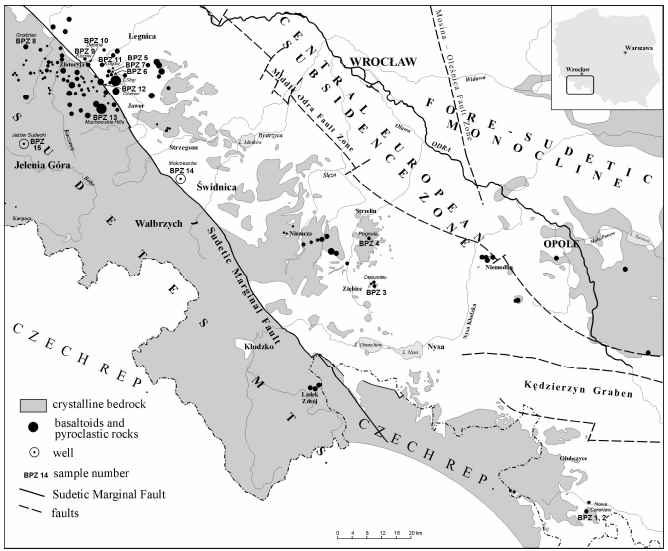
\includegraphics[width=0.7\linewidth]{../Termika/dslwulkanity}
 	\caption{Rozmieszczenie stanowisk występowania wulkanitów na Dolnym Śląsku; \textit{czarny} bazaltoidy i skały piroklastyczne, \textit{szary} podłoże krystaliczne \parencite{Badura.2005}.}
 	\label{badura}
 \end{figure}
 
 
 %Lanberger et al 2006  
 
 %stratygrafia wulkanitów dś na podst Birkenmajera
 
 %Wierzchołowski, 1993 --> geneza magm (BN) 
 %puziewicz 2011 - o płaszczu litosferycznym
 %http://www.geolodzy.uni.wroc.pl/bazalty/index.html
 
 
 
  	\section{Inwersja basenów przedpola} 
  
  %Nielsen et al., 2007
  %Mazur et al., 2005
 
  Pomiędzy pó\'{z}ną kredą a trzeciorzędem --- w trakcie orogenezy alpejskiej --- dalekosiężne oddziaływanie naprężeń generowanych na frontach kolizyjnych doprowadziło do inwersji morfologicznej basenów na przedpolach Alp i Karpat. Subdukcyjne zamknięcie basenu piemoncko-liguryjskiego w domenie wschodnioalpejskiej i w północnych Karpatach (w fazie eoalpejskiej w pó\'{z}nej kredzie; \cite{Lardeaux.1991}) skutkowało kolizją austroalpejskiego klinu orogenicznego z kontynentem europejskim, czego konsekwencją było wyniesienie Masywu Czeskiego oraz inwersja bruzdy śródpolskiej \parencite{Dezes.2004}.
  
  	\section{Południowy Bałtyk}
  	
  	%https://www.researchgate.net/publication/253713914_Genesis_of_high_intensity_intracratonic_heat_flow_anomalies_case_study_of_Western_Lithuania
  	
  	%https://www.nature.com/articles/ngeo261
  	
  	%http://engine.brgm.fr/web-offlines/Geothermal%20Field%20of%20The%20Baltic%20Region/index.html
  	
  	%https://www.sciencedirect.com/science/article/pii/004019519400215U
  	
Na obszarze państw bałtyckich obserwuje się rozległą pozytywną anomalię termiczną, której maksima występują w trzech miejscach \parencite{Lukosevicius.1993}:

\begin{itemize}
	\item w okolicach Jełgawy (Łotwa);
	\item na terenie obwodu kaliningradzkiego;
	\item w zachodniej części Litwy --- najbardziej intensywna i największa powierzchniowo anomalia.
\end{itemize}

\begin{figure}[h]
	\centering
	\fbox{\includegraphics[width=0.7\linewidth]{../../../Desktop/Termika/Grafika/Litwa_2}}
	\caption{\textit{Na górze} występowanie plutonów granitoidów mezoproterozoicznych w obrębie krystaliniku prekambryjskiego Litwy; \textit{ZN} --- intruzja Žemaičių Naumiestis; {na dole} rozkład izolinii powierzchniowego strumienia cieplnego (wartości w \si{\milli\watt\per\meter\squared}) na obszarze Litwy (na podstawie \cite{Sliaupa.2010})}
	\label{litwa}
\end{figure}

Anomalnie wysokie wartości strumienia cieplnego notowane na terenie zachodniej Litwy (ok. 15--30 km od wybrzeża między Kłajpedą a Szyłokarczmą; \cite{Lukosevicius.1993}; Fig. \ref{litwa}) sięgają 100 \si{\milli\watt\per\meter\squared} \parencite{Sliaupa.2012,Puura.2003}. Anomalia ta występuje na obszarze kratonu wschodnioeuropejskiego --- jednostki tego wieku typowo charakteryzują się niskimi wartościami parametrów termicznych \parencite{Suveizdis.2000}. Pod względem budowy geologicznej anomalia termiczna Kłajpedy znajduje się w miejscu występowania sigmoidy tektonicznej, powstałej przez zmianę kierunku strefy uskokowej Połock--Kurlandia i jej przejście w strefę tektoniczną Gotlandii (obie te struktury występują w obrębie podłoża kratonicznego; \parencite{Garetsky.2007}. Wysokie wartości strumienia cieplnego związane są z występowaniem kratonicznych intruzji granitoidowych mezoproterozoiku znacznej miąższości (w obrębie skał paleoproterozoicznych granulitowej domeny zachodniej Litwy), charakteryzujących się wysoką (rzędu 4--19 \si{\milli\watt\per\meter\cubic}) produkcją ciepła radiogenicznego \parencite{Sliaupa.2010,Sliaupa.2005,Motuza.2003}. Intruzje granitoidowe w obrębie prekambryjskiego krystaliniku Litwy (Fig. \ref{litwa}) powstały w fazie magmatyzmu, która nawiedziła południową część domeny bałtyckiej (również Bornholm, Gotlandię, Szwecję i północną Polskę) ok. 1,54--1,40 mln lat temu \parencite{Motuza.2008,Motuza.2006}. Temperatura w spągu największej intruzji Žemaičių Naumiestis sięga 95 \textcelsius \parencite{Sliaupa.2005}. Wspomniana intruzja powstała na przecięciu głębokiego uskoku Šilutė (Szyłokarczmy) o przebiegu W--E i strefy tektonicznej Niemna \parencite{Sliaupa.2005}. Gęstość strumienia cieplnego w obrębie anomalii zachodniolitewskiej waha się w granicach 55--100 \si{\milli\watt\per\meter\squared}, co wynika z heterogeniczności skał krustalnych i różnic w wytwarzaniu ciepła \parencite{Sliaupa.2005}. Nad plutonem Žemaičių Naumiestis strumień wynosi od 83 \si{\milli\watt\per\meter\squared} do 100 \si{\milli\watt\per\meter\squared} \parencite{Sliaupa.2005}. Za wysokie wartości strumienia cieplnego oprócz litologii skorupy odpowiadać musi dodatkowy czynnik, prawdopodobnie strumień cieplny od płaszcza jest na obszarze zachodniej Litwy wyższy niż typowo (12--15 \si{\milli\watt\per\meter\squared}) na kratonach \parencite{Motuza.2003}. Na obszarze paleoproterozoicznej granulitowej domeny zachodniolitewskiej notuje się płytkie zaleganie granicy MOHO (40--45 km; \cite{Sliaupa.2005,Suveizdis.2000}). Badania sejsmiczne wykazują istnienie strefy niskich prędkości (8,15--8,20 \si{\kilo\metre\per\second}) poniżej głębokości 60 km --- może to oznaczać obecność warunków wytapiania parcjalnego w tej strefie \parencite{Motuza.2003} lub istnienie kopułowatego wyniesienia płaszcza pod zachodnią Litwą \parencite{Janutyte.2014}. Przypuszcza się \parencite{Gordienko.1996}, że anomalia zachodniej Litwy może łączyć się z anomalią termiczną polskiego Pomorza i dalej na zachód z anomaliami występującymi na platformie paleozoicznej. Zasoby geotermiczne Litwy tworzą potencjał dla produkcji energii elektrycznej (np. \cite{Lukosevicius.1993,Sliaupa.2010}) --- w oparciu o ciepło zgromadzone w wodach podziemnych (dwa główne zbiorniki hydrogeotermalne: dewoński i kambryjski; \cite{Sliaupa.2012,Zinevicius.2010}) bąd\'{z} technologię HDR (ang. \textit{hot dry rock}; \cite{Sliaupa.2010}). 

Rejony podwyższonych wartości strumienia cieplnego na Litwie są powiązane nie tylko z występowaniem plutonów proterozoicznych, ale też (w mniejszym stopniu) z intruzjami fanerozoicznymi (permomezozoik). Należą do nich: zlokalizowany w północno-zachodniej części Litwy pluton Girkaliai oraz pola silli dolerytowych przy wybrzeżu litewskim i kaliningradzkim, wieku wczesnopermskiego \parencite{Motuza.2015}. W pó\'{z}nym paleozoiku mogło na Litwie dojść do znacznego (15--20 \si{\milli\watt\per\meter\squared} dla warstw kambru) zwiększenia strumienia cieplnego \parencite{Sliaupa.2006,Puura.2003}, w ramach mezozoicznego zdarzenia termicznego \parencite{Katinas.2004} na tym obszarze. 

\ct{spr Motuza et al., 2004}
\ct{kompleks mazurski - strumień cieplny?}

	\section{Diapiryzm płaszcza}

%https://books.google.pl/books?id=X4W9aGXDa9cC&pg=PA40&lpg=PA40&dq=vosges-black+forest+dome&source=bl&ots=BTjqrzht2G&sig=5T7J2u99LJTfjjOaLCNhscvkfd4&hl=pl&sa=X&ved=0ahUKEwiDg_CW4KjaAhULFCwKHSp1CtUQ6AEINjAF#v=onepage&q&f=false


Hipoteza piórpuszy (diapirów) płaszcza jest współcześnie często przyjmowana jako wytłumaczenie takich zjawisk z kenozoicznej historii geologicznej Europy, jak wulkanizm anorogeniczny na przedpolu Alp \parencite{Wilson.2001}, wynoszenie masywów waryscyjskich i powstanie systemu ryftów. W kontekście Europy środkowej mówi się o pióropuszach płaszcza, które miałyby być zlokalizowane pod basenem panońskim (np. \cite{Seghedi.2004}; \cite{Konecny.2002}) i pod Masywem Czeskim (np. \cite{Wilson.2001}). Duncan et al. (\citeyear{Duncan.1972}) sugerowali, że wulkanizm środkowoeuropejskiej prowincji kenozoicznej i paleogeńskiej prowincji północnoatlantyckiej mają \'{z}ródło w jednym pióropuszu płaszcza. Według koncepcji Duncan et al. (\citeyear{Duncan.1972}), zmiana lokalizacji wulkanizmu miałaby być związana z ruchem płyt litosferycznych, a także polarną rotacją płaszcza. Różne pola tektoniczne środkowoeuropejskiej prowincji wulkanicznej byłyby wówczas łańcuchem "wysp" wulkanicznych. Wykazano jednak, że nie potwierdza tego progresja czasowa wieku wulkanitów \parencite{Ritter.2001}. Badania Bijwaard i Spakman (\citeyear{Bijwaard.1999}) oraz Goes et al. (\citeyear{Goes.1999}) sugerują, że za stosunkowo młode zjawiska wulkaniczne w Europie kontynetalnej i współczesny wulkanizm Islandii może odpowiadać wykryta w badaniach sejsmicznych struktura płaszczowa. Bijwaard i Spakman (\citeyear{Bijwaard.1999}) postulują istnienie regionu niskich prędkości sejsmicznych o elipsoidalnym zarysie, na głębokościach ok. 900-1400 km (środkowy płaszcz). Region ten miałby się rozciągać od Islandii po Europę (np. Eifel, Masyw Centralny), masyw Ahaggar w Algierii, Wyspy Kanaryjskie i Wyspy Zielonego Przylądka, będąc \'{z}ródłem obecnych w tych miejscach pióropuszy płaszcza. Istnieją liczne prace potwierdzające (na podstawie badań sejsmicznych, geochemicznych i innych) istnienie tego typu zaburzeń konwekcyjnych w litosferze pod Europą (np. \cite{Ritter.2001}; \cite{Granet.1995}). Kompensacja notowanych wartości powierzchniowego strumienia cieplnego przy anomalii prędkości fal P i S w górnej astenosferze (do głębokości 200 km) Europy zachodniej i centralnej jest możliwa przy założeniu, że w litosferze obecne są ciała stopu. Ocenia się, że wspomniana anomalia zaczęła się rozwijać w paleocenie i odpowiada spągowi diapirów płaszcza \parencite{Dezes.2004}. Jednakże, część badaczy (np. \cite{Harangi.2007}; \cite{Plomerova.2007}) kwestionuje (w mniejszym lub większym stopniu), jakoby wytłumaczeniem dla wysokich wartości parametrów termicznych czy zjawisk wulkanicznych miałyby być proponowane diapiry płaszcza. Sugeruje się, że taki stan rzeczy jest raczej efektem procesów tektonicznych związanych z ruchami płyt tektonicznych \parencite{Harangi.2007}. 

%zajrzeć do Dezes.2004

\chapter{Modele termiczne dla obszaru Polski --- historia badań}

\section{Pierwsze oznaczenia wartości parametrów geotermicznych dla ziem polskich}

Pierwsze pomiary parametrów geotermicznych w otworach wiertniczych (temperatury, T, gradientu, dT/dz, i stopnia geotermicznego, dz/dT) na terenach polskich wykonywane były przez badaczy niemieckich na Górnym Śląsku w początkach XX w. W \citeyear{Henrich.1904} r. opublikowane zostały wyniki obserwacji termicznych Henricha poczynionych na odwiercie Paruschowitz V (w literaturze polskiej: Paruszowiec lub Paruszowice; np. \cite{Plewa.1966,Stenz.1936}) w Rybniku. Uzyskano wówczas (po przyjęciu poprawek) gradient termiczny 31,8 m/{\textcelsius}. Jest to jednak wynik wysoce niepewny, gdyż mierzono temperaturę rdzeni skalnych wydobytych na powierzchnię \parencite{Maj.2010,Rudzki.1909,Henrich.1904}. Michael i Quitzow (\citeyear{Michael.1910}) prowadzili badania na otworze Czuchów (dziś w dzielnicy Czerwionki--Leszczyn). Temperatury mierzono przy użyciu termometrów zapuszczanych do otworów (Fig. \ref{michael}; \cite{Michael.1910}). Arctowski \parencite{Arctowski.1923a} pisał, że były to badania ,,pełne błędów''. W latach 20. XX w. licznymi badaniami na polu geoftermiki zaznaczył się ośrodek lwowski pod wodzą prof. H. Arctowskiego \parencite{Plewa.1966,Maj.2010}. Po II wojnie światowej badania geofizyczne w otworach wiertniczych, a wśród nich badania termiczne, znalazły się w fazie intensywnego rozwoju \parencite{Plewa.1994}. Pomiary temperatur w odwiertach przeprowadzane były również w pó\'{z}niejszch dekadach, m. in. w latach 50. i 60. przez E. Stenza, St. Pawłowskiego \ct{(Łeba)}, St. Plewę, St. Depowskiego i L. Romana (Magnuszew IG-1) \parencite{Plewa.1966,Roman.1962,Stenz.1936}. \ct{dopisac gdzie były badania} Punktowe oznaczenia strumienia cieplnego wykonywali: Stenz \ct{\citeyear{Stenz.1954}} (1,23 \si[sticky-per]{\micro\calorie.cm^{-2}.s^{-1}} dla otworu Ciechocinek) oraz Plewa \ct{parencite{Plewa.1961,Plewa.1963a,Plewa.1963b,Plewa.1965,Plewa.1966}}. 

\begin{figure}[h]
	\centering
	\includegraphics[width=0.6\linewidth]{../../../Desktop/Termika/Grafika/Michaelv2}
	\caption{Średnie wartości pomiarów temperatury w otworze Czuchów \parencite{Michael.1910}}
	\label{michael}
\end{figure}
	
\subsubsection{Prace Arctowskiego i in. (lata 20. XX w.)}

W latach 20. XX w. (od 1922; \cite{Olpinska.1988}) H. Arctowski, dyrektor Instytutu Geofizyki i Meteorologii Uniwersytetu Jana Kazimierza we Lwowie, koordynował prace badawcze z zakresu geotermii na ok. 150 otworach wiertniczych ropy naftowej na Podkarpaciu \parencite{Maj.2010,Olpinska.1988}. Wyniki owych pomiarów (Tab. \ref{arctowski}), jak i opisy procedury pomiarowej były wielokrotnie publikowane (m. in. \cite{Arctowski.1923c,Arctowski.1923b,Arctowski.1923a}). Arctowski samodzielnie opracował technikę pomiaru temperatur w otworach, eksperymentował z wykorzystaniem różnych termometrów. Pomiary temperatur przeprowadzano na różnych głębokościach (co 20--50 m), z jednoczesnym zastosowaniem trzech termometrów lekarskich maksymalnych, umieszczonych w obciążonej szklanej probówce zatopionej od góry parafiną. Probówkę zapuszczano do otworu na lince stalowej o średnicy 1 mm.Temperatury mierzono w nocy, podczas przerw w wierceniach. Działalność naukową Instytutu przerwał wybuch wojny, wskutek czego wielu z prac nie ukończono i nie opublikowano \parencite{Olpinska.1988}. Arctowski w swoich pracach rozważał możliwe czynniki zakłócające pomiar, takie jak: temperatura na powierzchni, wpływ cyrkulacji wód podziemnych itp. S. Zych i J. Moniak, należący do współpracowników H. Arctowskiego, również prowadzili w końcu lat 20. prace geotermiczne, m. in. przy poszukiwaniu gorących solanek w Ciechocinku \parencite{Maj.2010}.

%Wartości parametrów geotermicznych wyznaczone w pracach Arctowskiego (\citeyear{Arctowski.1923b,Arctowski.1923a}); \textit{Z} --- głębokość otworu, \textit{z} --- głębokość pomiaru, \textit{H} --- stopień geotermiczny, \textit{b.d.} --- brak danych

\begin{sidewaystable}[h]
	\centering
	\caption{Wartości temperatury i stopnia geotermicznego wyznaczone w pracach Arctowskiego \citeyear{Arctowski.1923b,Arctowski.1923a}; \textit{Z} --- głębokość odwiertu, \textit{z} --- głębokość pomiaru, \textit{H} --- stopień geotermiczny, \textit{b.d.} --- brak danych}
	\label{arctowski}
		\begin{tabular}{llllllll}
		\hline
		Źródło & Miejsce & Odwiert & Stan odwiertu & Z [m] & z [m] & T [\textcelsius] & H [m{\textcelsius}^{-1}] \\ \hline
		&  & \cellcolor[HTML]{EFEFEF} & \cellcolor[HTML]{EFEFEF} & \cellcolor[HTML]{EFEFEF} & \cellcolor[HTML]{EFEFEF}50 & \cellcolor[HTML]{EFEFEF}8,3 & \cellcolor[HTML]{EFEFEF} \\
		&  & \cellcolor[HTML]{EFEFEF} & \cellcolor[HTML]{EFEFEF} & \cellcolor[HTML]{EFEFEF} & \cellcolor[HTML]{EFEFEF}200 & \cellcolor[HTML]{EFEFEF}12,1 & \cellcolor[HTML]{EFEFEF} \\
		&  & \cellcolor[HTML]{EFEFEF} & \cellcolor[HTML]{EFEFEF} & \cellcolor[HTML]{EFEFEF} & \cellcolor[HTML]{EFEFEF}750 & \cellcolor[HTML]{EFEFEF}22,3 & \cellcolor[HTML]{EFEFEF} \\
		&  & \cellcolor[HTML]{EFEFEF} & \cellcolor[HTML]{EFEFEF} & \cellcolor[HTML]{EFEFEF} & \cellcolor[HTML]{EFEFEF}880 & \cellcolor[HTML]{EFEFEF}25,6 & \cellcolor[HTML]{EFEFEF} \\
		&  & \multirow{-5}{*}{\cellcolor[HTML]{EFEFEF}Prezydent No 1.} & \multirow{-5}{*}{\cellcolor[HTML]{EFEFEF}W trakcie wiercenia} & \multirow{-5}{*}{\cellcolor[HTML]{EFEFEF}926} & \cellcolor[HTML]{EFEFEF}921 & \cellcolor[HTML]{EFEFEF}24,7 & \multirow{-5}{*}{\cellcolor[HTML]{EFEFEF}\makecell{53,9(750--200 m), \\ 48,0 (880--50 m), \\ 39,4 (220--50 m \\ i 880--750 m)}} \\
		&  & Mougeot No 2. & 2--tyg. stójka & 772 & 50 & 7,9 & b.d. \\
		&  & \cellcolor[HTML]{EFEFEF} & \cellcolor[HTML]{EFEFEF} & \cellcolor[HTML]{EFEFEF} & \cellcolor[HTML]{EFEFEF}50 & \cellcolor[HTML]{EFEFEF}7,5 & \cellcolor[HTML]{EFEFEF} \\
		&  & \cellcolor[HTML]{EFEFEF} & \cellcolor[HTML]{EFEFEF} & \cellcolor[HTML]{EFEFEF} & \cellcolor[HTML]{EFEFEF}250 & \cellcolor[HTML]{EFEFEF}11,0 & \cellcolor[HTML]{EFEFEF} \\
		\multirow{-9}{*}{Arctowski, 1923a} & \multirow{-9}{*}{Bitków} & \multirow{-3}{*}{\cellcolor[HTML]{EFEFEF}Valotte No 3.} & \multirow{-3}{*}{\cellcolor[HTML]{EFEFEF}Wiercenie przerwane} & \multirow{-3}{*}{\cellcolor[HTML]{EFEFEF}407} & \cellcolor[HTML]{EFEFEF}350 & \cellcolor[HTML]{EFEFEF}12,8 & \multirow{-3}{*}{\cellcolor[HTML]{EFEFEF}56,6} \\
		&  &  &  &  & 10 & 9,6 &  \\
		&  &  &  &  & 25 & 9,7 &  \\
		&  &  &  &  & 70 & 9,7 &  \\
		&  &  &  &  & 75 & 10,0 &  \\
		&  &  &  &  & 100 & 10,5 &  \\
		&  &  &  &  & 150 & 11,6 &  \\
		&  &  &  &  & 200 & 12,5 &  \\
		&  &  &  &  & 250 & 13,6 &  \\
		\multirow{-9}{*}{Arctowski, 1923b} & \multirow{-9}{*}{Borysław} & \multirow{-9}{*}{Ratoczyn 5} & \multirow{-9}{*}{Odwiert opuszczony} & \multirow{-9}{*}{b.d.} & 300 & 14,4 & \multirow{-9}{*}{b.d.} \\ \hline
	\end{tabular}
\end{sidewaystable}

\section{Rys historyczny modelowania termiki obszaru Polski}

Pierwsze znaczące publikacje z zakresu modelowania termiki obszaru Polski --- wyznaczania wartości parametrów geotermicznych i obrazowania ich przestrzennej oraz wgłębnej zmienności --- powstały po II wojnie światowej. Szczegółowe rozpoznanie charakterystyki geotermicznej przeprowadzano na obszarach górniczych węgla (od lat 50., \parencite{bibid}) i miedzi (od lat 60., \parencite{bibid}). 

\subsubsection{Różycki, 1948. \textit{Uwagi o rozmieszczeniu stopnia geotermicznego w Polsce i w krajach sąsiednich}} \nocite{Rozycki.1948}
Notatka z referatu wygłoszonego w 1947 r. zawiera skrótowy opis poglądów Różyckiego na charakterystykę geotermiczną powierzchni kraju. Różycki wskazuje na dużą zmienność wielkości geotermicznych na terenie Polski. Jednocześnie zwraca uwagę na skąpy stan i niepewną wiarygodność dotychczasowych badań dla obszaru Polski (wzmiankowane badania Arctowskiego i jego uczniów; \ct{cite{bibid}}), pozwalające jedynie na wstępną i szkicową syntezę zebranych danych. Autor wyróżnia kilka regionów geotermicznych górnej litosfery w Polsce, mając na względzie ich historię tektoniczną (określenia w cudzysłowach za \cite{Rozycki.1948}):
 \begin{itemize}%[nolistsep]
 	\item Polska północno-wschodnia --- region ,,chłodny'' (stopień geotermiczny: 40--100 m); obszar kratoniczny;
 	\item Polska południowa i południowo--zachodnia --- region ,,przeciętnie ciepły'' (średni stopień geotermiczny: 30--40 m); strefa fałdowań hercyjskich i kimeryjskich oraz zapadlisko przedkarpackie;
 	\item obszar karpacki --- region ,,nieco ochłodzony'' (stopień geotermiczny: 40--45 m);
 	\item Masyw Czeski --- region ,,miernie chłodny'' (stopień geotermiczny: 40--55 m);
 	\item strefy wulkanizmu trzeciorzędowego i związane z nimi ,,lokalne ocieplenia'';
 	\item zaplecze Karpat --- region ,,ciepły''; strefa ,,głębokich rozdarć tektonicznych w wewnętrznej części łuku Karpat''.
 \end{itemize}
Ponadto, Różycki podkreśla, że przebieg strefy Teisseyre'a--Tornquista (będącej granicą między obszarami o różnym wieku) znajduje odzwierciedlenie w rozmieszczeniu izolinii średniego stopnia geotermicznego na obszarze Polski.
 
W zbiorze opublikowano szkicową mapę rozmieszczenia średniego stopnia geotermicznego w Polsce wraz z miejscami i wartościami pomiarów z ważniejszych wierceń (Fig. \ref{rozycki}). Została ona opracowana na podstawie danych z otworów: Łeba, Pisz, Szubin, Aleksandrów, Paruszowiec i Krosno, oraz wartości pomierzonych w odwiertach w krajach ościennych \parencite{Plewa.1966}. Dane, których użył Różycki dla otworów: Pisz i Łeba były zawyżone względem rzeczywistych wartości, co wpłynęło na nieprawidłowy rozkład gradientu geotermicznego dla Polski północno--wschodniej na zamieszczonej w publikacji mapie \parencite{Stenz.1954}. Rozdzielczość przestrzenna danych, na podstawie których skonstruowano mapę, była niska (zwłaszcza poza obszarami nawiercanymi dla celów naftowych), przez co otrzymany model rozkładu geoterm mógł być jedynie szkicowy. Praca Różyckiego stała się punktem wyjścia odniesieniem dla pó\'{z}niejszych badaczy termiki litosfery (np. \cite{Plewa.1966,Majorowicz.1971}).

\begin{figure}[h]
	\centering
	\fbox{\includegraphics[width=0.7\linewidth]{../../../Desktop/Termika/Grafika/rozycki}}
	\caption{Mapa rozkładu izolinii stopnia geotermicznego w Polsce (wg \cite{Rozycki.1948})}
	\label{rozycki}
\end{figure}
	
\subsubsection{Plewa, 1966. \textit{Regionalny obraz parametrów geotermicznych obszaru Polski}}
Praca Plewy z 1966 r. zawiera zestawienie danych geotermicznych (stopnia i gradientu geotermicznego) dla 27 otworów, w tym 11 opisanych we wcześniejszej literaturze. Publikowane pomiary były zbierane od 1953 r.; autor wykonywał również w ramach swoich wcześniejszych prac oznaczenia stopnia geotermicznego i strumienia cieplnego w wybranych miejscach Polski oraz badania własności termicznych skał \ct{parencite{Plewa.1961,Plewa.1963a,Plewa.1963b,Plewa.1965}}. Zamieszczono mapę rozkładu gradientu geotermicznego na obszarze Polski, opracowaną z wykorzystaniem wielomianów 1., 2. i 3. stopnia. Obliczenia wykonano w Katedrze Geodezji Wyższej i Obliczeń Geodezyjnych Akademii Górniczo-Hutniczej na matematycznej maszynie cyfrowej, dla różnych przedziałów głębokości. Autor stwierdził ogólną zgodność swoich wyników (dla modelu uzyskanego w oparciu o wielomian 3. stopnia) z mapą Różyckiego \citeyear{Rozycki.1948}. 

W publikacji przedstawiono wartości powierzchniowego strumienia cieplnego ziemi dla 6 otworów wiertniczych z obszaru Polski (Tab. \ref{plewa}), na podstawie oznaczonych w wierceniach wartości gradientu geotermicznego i oporności cieplnej skał pobranych z rdzeni. W pracy znajdują się również rozdziały poświęcone teorii i praktyce pomiarów geotermicznych w otworach i na próbkach rdzeni. 

\begin{table}[h]
	\centering
	\caption{Średnie wartości gęstości strumienia cieplnego dla otworów opisanych w pracy \cite{Plewa.1966}; ${}^{1}$ --- brak stabilności termicznej podczas pomiaru \parencite{Plewa.1994}, ${}^{2}$ --- wartość q zaniżona --- zaniżona wartość przewodności właściwej, $\lambda$, mierzonej na próbkach poddanych wieloletniemu wpływowi czynników atmosferycznych \parencite{Plewa.1994}, ${}^{3}$ --- G i $\lambda$ zmienne z głębokością \parencite{Plewa.1966}}
	\label{plewa}
	\begin{tabular}{@{}lllll@{}}
		\toprule
		Lp. & Nazwa otworu     & G    & $\lambda$ & q    \\ \midrule
		1   & Bartoszyce IG--1 & 1,54 & 0,0052                 & 0,80 \\
		2   & Mielnik IG--1    & {1,64}^{1} & 0,0054                 & 0,89 \\
		3   & Wschowa 1        & 3,05 & 0,0056                 & 1,71 \\
		4   & Ostrzeszów 1     & 2,22 & 0,0060                 & 1,33 \\
		5   & Żółcza 1        & 3,45 & {0,0032?}^{2}                & 1,10 \\

		6   & Zakopane IG--1   & {}^{3}    & {}^{3}                      & 1,33 \\ \bottomrule
	\end{tabular}
\end{table}

\subsubsection{Majorowicz, 1971. \textit{Przebieg wartości stopnia geotermicznego w Polsce w przedziale głębokości 200--2500 m} i pó\'{z}niejsze prace Majorowicza}
Począwszy od lat 70. XX w. J. Majorowicz przedstawił (samodzielnie bądź we współautorstwie) szereg prac na temat charakterystyki geotermicznej obszaru Polski. Pierwsza z nich ukazała się w roku 1971. W publikacji zamieszczono wartości gradientu i stopnia geotermicznego dla 22 otworów z obszaru Polski (w tym 10 na podstawie nowych pomiarów), w których przeprowadzono dokładne oznaczenia termiczne. Wartości H i G podano w uśrednieniu dla przedzialu głębokości 200--2500 m. Zdaniem Majorowicza, taki zabieg umożliwił korelację uzyskanych wartości z rzeźbą podłoża krystalicznego na danym obszarze. W oparciu o ustalone wartości H wykonano (metodą interpolacji graficznej) mapę przebiegu izolinii stopnia geotermicznego w Polsce w przedziale 200--2500 m. Majorowicz odnotował, że omawiana mapa wykazuje dużą zbieżność z mapą wartości H dla przedziału 200--2000 m, zaproponowaną w pracy Plewy (\citeyear{Plewa.1966}).

\subsubsection{Węsierska, 1973. \textit{A study of terrestial heat flux density in Poland}} 

\subsubsection{Motyl-Rakowska i Sokołowski, 1980. \textit{Temperatures at the base of the Permian-Cainozoic stratum in Poland}}

\subsubsection{Plewa, \citeyear{Plewa.1994}. \textit{Rozkład parametrów geotermalnych na obszarze Polski} i wcześniejsze prace Plewy}

Publikacja powstała jako część grantu pt. ,,Badanie rozkładu parametrów geotermicznych wybranych obszarów górniczych'', realizowanego w latach 1992--1994. W pracy znajdują się rozdziały poświęcone rozkładowi pola termicznego i cieplnego na obszarze Polski. Zamieszczono wyniki licznych badań otworowych temperatury (wraz z krytycznym omówieniem) oraz mapy izoterm na różnych głębokościach, skonstruowane w oparciu o dane z otworów (z Polski i krajów sąsiednich), dla których wyznaczano strumień cieplny Ziemi. Wartości strumienia cieplnego pomierzone w otworach na terytorium Polski zebrano w formie tabeli, mieszczącej 87 pozycji z 84 przebadanych otworów (w 3 z otworów wartość q wyznaczano dwukrotnie). Wzmiankowane oznaczenia strumienia cieplnego stały się podstawą dla wykonania umieszczonej i opisanej w pracy mapy izolinii strumienia cieplnego na obszarze Polski. Książka zawiera obszerne omówienie właściwości termicznych skał osadowych występujących w podłożu poszczególnych regionów Polski, ze szczególnym odniesieniem do obszarów górniczych. Opisano również skały z terenu Polski pod względem generowanego ciepłą radiogenicznego.

\subsubsection{Gordienko i Zavgorodnyaya, \citeyear{Gordienko.1996}. \textit{Estimation of heat flow in Poland}}

W pracy zamieszczono wykaz wartości strumienia cieplnego dla 176 otworów z obszaru Polski (w tym 11, w których strumień cieplny oznaczano po raz pierwszy). Załączono mapę, sporządzoną na podstawie tych wartości. Autorzy szczególną uwagę poświęcili anomaliom termicznym obserwowanym na obszarze Polski. Wymieniono następujące dodatnie anomalie termiczne:

\begin{itemize}
\item \textbf{Pomorze} (na Bałtyku przy wybrzeżu polskim) --- anomalia związana ze strefą aktywności sejsmicznej Rymań--Karlino--Manowo \ct{Karlin czy Karlino? - spr. w Pagaczewski};
\item subpołudnikowa anomalia \textbf{basenu Odry} i anomalia \textbf{basenu Warty}, połączone od południa subrównoleżnikową anomalią w osi \textbf{Radom--Wrocław--Praga};
\item przypuszczalna subrównoleżnikowa anomalia na \textbf{przedpolu Karpat};
\item niewielka anomalia \textbf{Chełma} i możliwe przedłużenie anomalii \textbf{Jaworowa (okręg lwowski)} na obszar Polski. 
\end{itemize}

Gordienko i Zavgorodnyaya wskazują na czynniki zaburzające wartości strumienia cieplnego na powierzchni, takie jak przepływ wód podziemnych i rze\'{z}ba terenu. We wnioskach zwracają uwagę na potrzebę uszczegółowienia danych na temat strumienia cieplnego w Polsce, dzięki czemu możliwe byłoby dokładniejsze oznaczenie anomalii termicznej i ich ocena na tle regionalnej historii geologicznej. Autorzy postulują, by (pod warunkiem większej rozdzielczości danych) skonstruować trójwymiarowy model termiczny polskiej tektonosfery.

\subsubsection{Karwasiecka i Bruszewska, 1997. \textit{Gęstość powierzchniowego strumienia cieplnego ziemi na obszarze Polski}}

\iffalse
do znalezienia: 

Motyl-Rakowska, J., Sokolowski, J.
Temperatures at the base of the Permian-Cainozoic stratum in Poland
(1980) Publs. Inst. Geophys. Pol. Acad. Sc., A-8 (130), pp. 51-54. Cited 1 time.


Plewa, M., Plewa, S., Poprawa, D., Tomas, A.
Geothermal Atlas of Europe
(1992) Her. Haack Verl., Potsdam, null p. Cited 1 time.

 Prace Instytutu GeologicznegoVolume 106, 1983, 88p
( Geothermics of the copper ore deposit of the Fore-Sudetic monocline).(Article)
[Geotermika ziozo rud miedzi monokliny przedsudeckiej.]
Downorowicz, S. 

 Karwaaiecka M.l  Atlas geologiczny Górnośląskiego  Zagłębia Węglowego. 
Wyd.  Geologiczne,  Warszawa  1980.

Wȩsierska, M.
A study of terrestial heat flux density in Poland
(1973) Publ. Inst. Geophys. Pol. Acad. Sc. (Materialy i Prace), 60, pp. 135-144. Cited 2 times. (G0, 135)

KARWASIECKA M. i BRUSZEWSKA B. 1997 — Gestosc
powierzchniowego strumienia cieplnego ziemi na obszarze Polski.
CAG Pañstw. Inst. Geol., nr 060 21/98
\fi

\chapter{Rozpoznanie strumienia cieplnego na obszarze Polski}

\chapter{Teoretyczne podstawy modelowania stanu termicznego litosfery}

%Plewa, 1994

\chapter{Parametry materiałowe skał}

%Plewa, 1994

\chapter{Rozpoznanie struktury litosfery na obszarze Polski}

\section{Wielkie eksperymenty sejsmiczne}

Profilowanie sejsmiczne jako metoda badania głębokiej struktury litosfery było wykorzystywane w Polsce od lat 60. XX w. \ct{zrodlo}. Na przestrzeni ostatnich dwóch dekad przeprowadzono na obszarze Polski kilka wielkoskalowych eksperymentów sejsmicznych:

\subsubsection{POLONAISE'97}
Eksperyment głębokich sondowań sejsmicznych POLONAISE'97 przeprowadzono w roku 1997 w celu rozpoznania struktury tektonicznej (i jej ewolucji ku północnemu zachodowi) polskiego segmentu TESZ oraz zachodniego krańca EEC \parencite{GrupaRoboczaPOLONAISE.2002}. W ramach badań wykonywano również rozpoznanie sejsmiczne wypełnienia osadowego basenu polskiego \parencite{GrupaRoboczaPOLONAISE.2002}. Dane zbierano wzdłuż 5 profili o łącznej długości ok. 2000 km \parencite{GrupaRoboczaPOLONAISE.2002}. Zastosowanie kilku profili umożliwiło pozyskanie danych o budowie wgłębnej badanego obszaru w 3D \parencite{Guterch.1998}.

%https://www.pgi.gov.pl/projekt-polonaise/9998-projekt-polonaise.html
%PASSEQ 2006--2008
%POLONAISE'97
%CELEBRATION 2000
%POLCRUST
%PolandSPAN™

\section{Struktura litosfery na obszarze Polski}

\subsection{Strefa TESZ}
TESZ (z ang. \textit{Trans-European Suture Zone}) jest szeroką strefą deformacji powaryscyjskich, która powstała w miejscu akrecji terranów egzotycznych (gondwańskich) do krawędzi Baltiki \parencite{Belka.2002,Guterch.1998}. Terrany dokowały do zachodniej krawędzi kratonu prekambryjskiego, równolegle do linii Teisseyre'a-Tornquista \parencite{Belka.2002}. Lineament TT nie odpowiada jednak bezpośrednio granicy między Avalonią a Baltiką \parencite{Mizerski.2017,Mazur.2015}. Strefa TESZ rozciąga się od Wysp Brytyjskich na północnym zachodzie po rejon Morza Czarnego na południowym wschodzie \parencite{Guterch.1998}. 

Strefa TESZ wpłynęła na rozwój tektoniczny młodszych warstw skorupy --- na jej obszarze rozwinął się w permie głęboki basen sedymentacyjny pokrywający dużą część Polski i północnych Niemiec, określany mianem basenu polskiego (rejon basenu środkowoeuropejskiego; \cite{Guterch.1998}). W czasie orogenezy alpejskiej doszło do inwersji TESZ i powstania SE--NW pasa wyniesień wzdłuż strefy TT \parencite{Guterch.1998}.

Poznanie szczegółow budowy podłoża w północnej części strefy TESZ w Polsce (z mniejszą liczbą wychodni i wierceń, niż część południowa) jest utrudnione przez znaczną miąższość pokrywy osadowej górnego paleozoiku, mezozoiku i czwartorzędu \parencite{Belka.2002}. Szczególną przeszkodę stanowią pokłady soli permskich, absorbujących sygnał sejsmiczny \parencite{Guterch.1998}. W południowej części Polski dobrze poświadczone są trzy terrany gondwańskie: strefy TESZ --- bloki: łysogórski, małopolski i górnośląski (lub Brunovistulicum, \cite{Bula.2008,Belka.2002}). Ogólnie rzecz biorąc, pod względem sejsmicznym strefa TT dzieli obszar Polski na rejon wysokich prędkości na północnym wschodzie (EEC) i strefę niskich prędkości na południowym zachodzie (platforma paleozoiczna; \cite{Guterch.1998}). Badania sejsmiczne wzdłuż profilu LT-7 w północno-zachodniej Polsce wykazały, że grubość skorupy w rejonie TESZ jest pośrednia między skorupą kratoniczną EEC wschodniej Polski a skorupą platformową Polski zachodniej \parencite{Guterch.1994}. 

\chapter{Ocena perspektyw modelowania stanu termicznego litosfery na obszarze Polski}

\renewcommand\headrulewidth{0pt} %usuwa linie w nagłówku
{\renewcommand{\markboth}[2]{} %usuwa tekst nagłówka
	\printbibliography[heading=bibintoc,title=Bibliografia]} %[minnames=1,maxnames=99]

\end{document}
